\documentclass[12pt]{article}

\usepackage{tabularx}
\usepackage[a4paper,margin=2.5cm, bottom=2.5cm]{geometry}
\usepackage{fancyhdr}
\usepackage{listings}
\usepackage{booktabs}
\usepackage{float}
\usepackage{subcaption}
% \usepackage{caption}
% \captionsetup{font=footnotesize}
\usepackage{graphicx}
\usepackage{amsmath}
\usepackage{amssymb}
\usepackage{amsthm}
\usepackage{array}
\usepackage[table]{xcolor}
\usepackage{pgfplots}
\pgfplotsset{compat=1.17}
\usepackage{pgfplotstable}
\usepackage{multirow}
\usepackage{tikz}
\usepackage[hidelinks]{hyperref}
\usepackage{titling}
\usepackage[polish]{babel} % Polish language support

\setlength{\headheight}{40pt}
\setlength{\parindent}{0pt}
\setlength{\parskip}{1ex}
\renewcommand{\headrulewidth}{0pt}

\pagestyle{fancy}
\fancyhead{}
\fancyhead[L]{
    \renewcommand{\arraystretch}{1.5}
    \begin{tabularx}{\textwidth}{|X|X|}
        \hline
        \bfseries Obliczenia inteligentne & \bfseries \thetitle \\
        \hline
    \end{tabularx}
}
\fancyfoot[C]{\thepage}

\renewcommand{\maketitle}{
    \thispagestyle{plain}
    \renewcommand{\arraystretch}{2}
    \vspace*{-8em}
    \footnotesize
    \begin{flushleft}
        \begin{tabularx}{\textwidth}{|X|X|}
            \hline
            \bfseries Obliczenia Inteligentne  & \bfseries \thetitle                           \\ \hline
            \multicolumn{2}{|l|}{
                \begin{tabular}[t]{@{}ll@{}} 
                    \textbf{Grupa:} Grupa 1
                    \hspace{4.5em}
                    \textbf{Dzień i czas:} Czwartek, 10:00
                    \hspace{4.5em}
                    \textbf{Rok akademicki:} 2023/24
                \end{tabular}
            } \\ \hline
            \multicolumn{2}{|l|}{
                \begin{tabular}[t]{@{}l@{\hspace{10em}}l@{}} 
                    \textbf{Imię i nazwisko:} \textsc{Jakub Pawlak} & \textbf{Imię i nazwisko:} \textsc{Magdalena Paku\l a} 
                \end{tabular}
            } \\
            \hline
        \end{tabularx}
    \end{flushleft}
    \renewcommand{\arraystretch}{1}
}


\usepackage{pgfplotstable}
\title{Projekt 1 - Zadanie 2}

\newcommand*{\subfigwidth}{0.24\textwidth}

\begin{document}
\maketitle

\begin{figure}[H]\centering
    \begin{subfigure}[t]{\subfigwidth}
        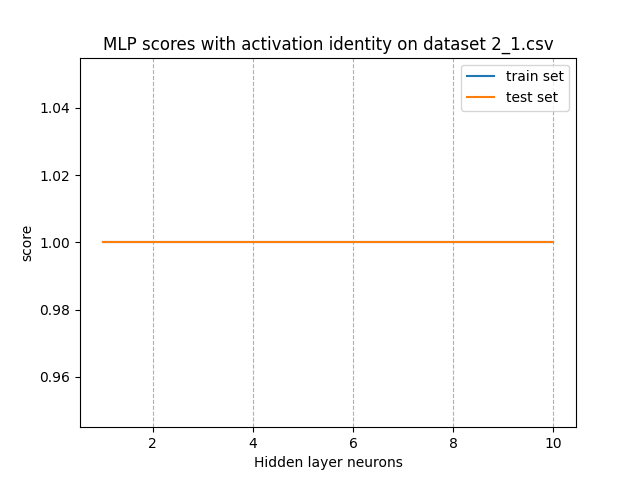
\includegraphics[width=\linewidth]{img/exp_1/mlp/2_1/identity/scores.png}
        \caption{identity 2\_1}
    \end{subfigure}
    \hfill
    \begin{subfigure}[t]{\subfigwidth}
        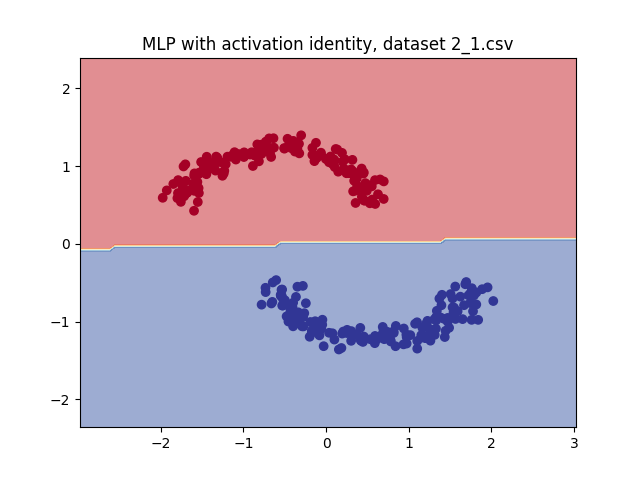
\includegraphics[width=\linewidth]{img/exp_1/mlp/2_1/identity/boundary.png}
        \caption{identity 2\_1}
    \end{subfigure}
    \hfill
    \begin{subfigure}[t]{\subfigwidth}
        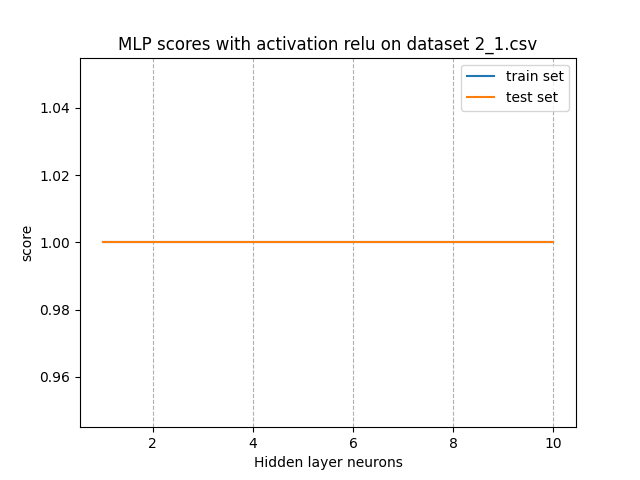
\includegraphics[width=\linewidth]{img/exp_1/mlp/2_1/relu/scores.png}
        \caption{ReLu 2\_1}
    \end{subfigure}
    \hfill
    \begin{subfigure}[t]{\subfigwidth}
        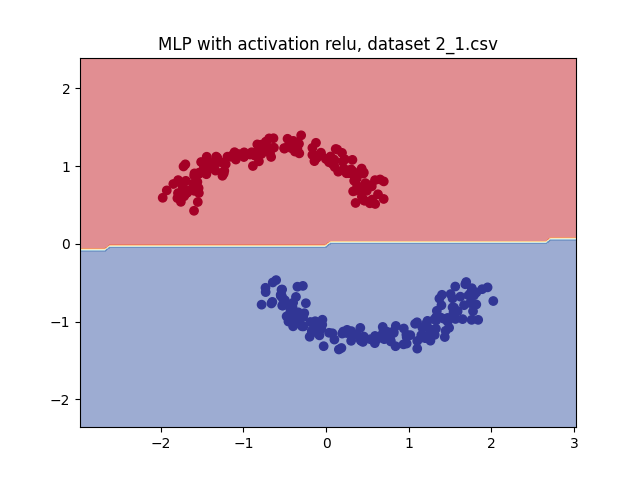
\includegraphics[width=\linewidth]{img/exp_1/mlp/2_1/relu/boundary.png}
        \caption{ReLu 2\_1}
    \end{subfigure}
    \\
    \begin{subfigure}[t]{\subfigwidth}
        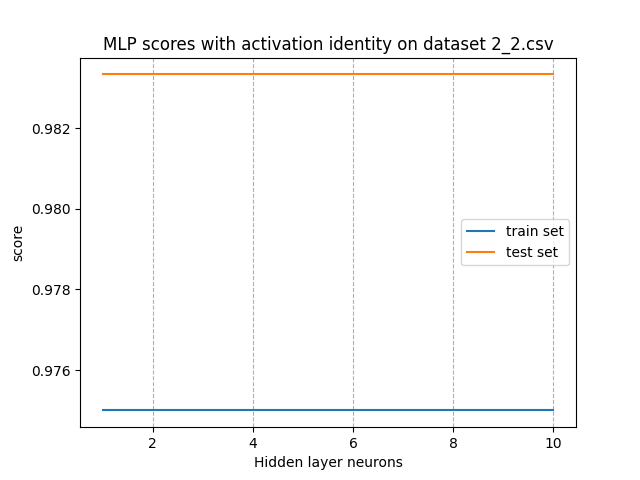
\includegraphics[width=\linewidth]{img/exp_1/mlp/2_2/identity/scores.png}
        \caption{identity 2\_2}
    \end{subfigure}
    \hfill
    \begin{subfigure}[t]{\subfigwidth}
        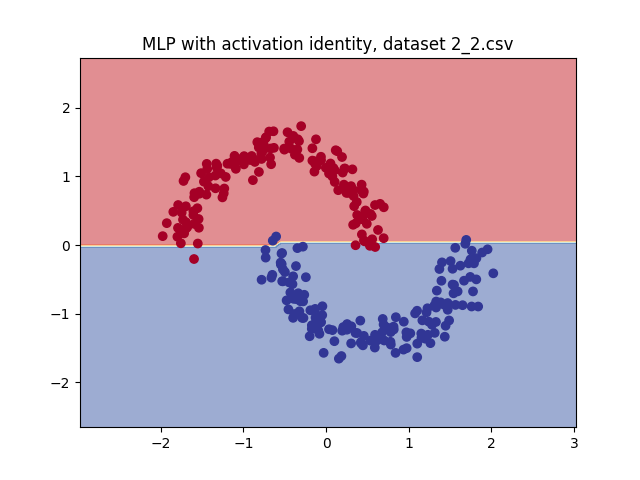
\includegraphics[width=\linewidth]{img/exp_1/mlp/2_2/identity/boundary.png}
        \caption{identity 2\_2}
    \end{subfigure}
    \hfill
    \begin{subfigure}[t]{\subfigwidth}
        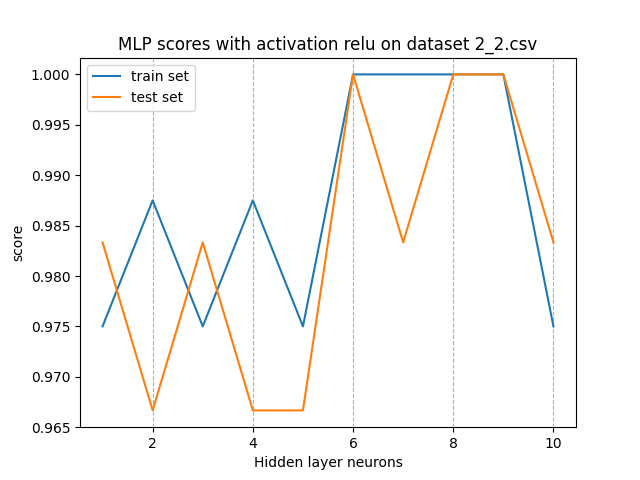
\includegraphics[width=\linewidth]{img/exp_1/mlp/2_2/relu/scores.png}
        \caption{ReLu 2\_2}
    \end{subfigure}
    \hfill
    \begin{subfigure}[t]{\subfigwidth}
        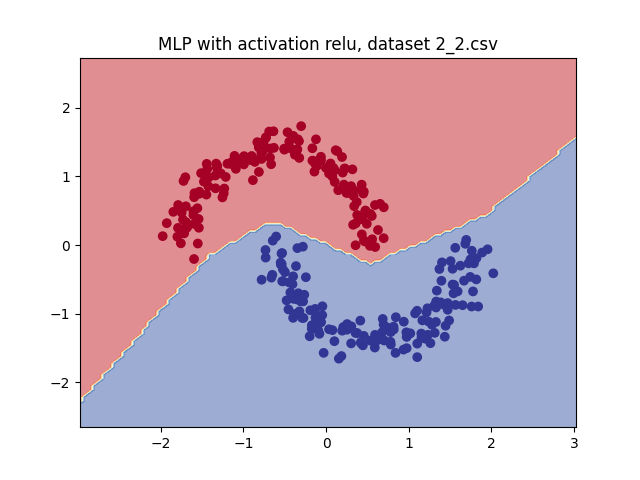
\includegraphics[width=\linewidth]{img/exp_1/mlp/2_2/relu/boundary.png}
        \caption{ReLu 2\_2}
    \end{subfigure}
    \\
    \begin{subfigure}[t]{\subfigwidth}
        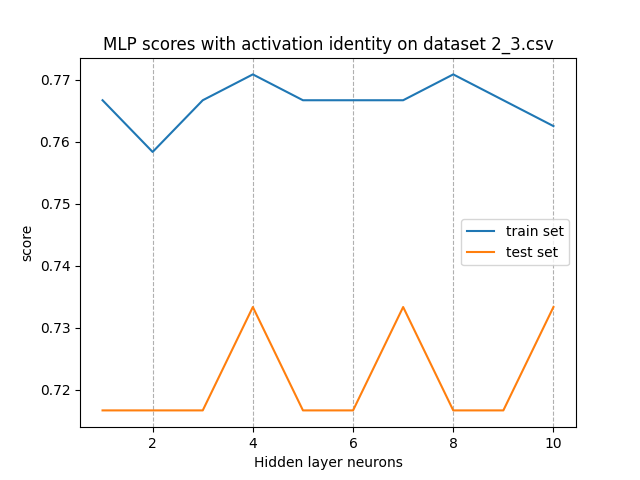
\includegraphics[width=\linewidth]{img/exp_1/mlp/2_3/identity/scores.png}
        \caption{identity 2\_3}
    \end{subfigure}
    \hfill
    \begin{subfigure}[t]{\subfigwidth}
        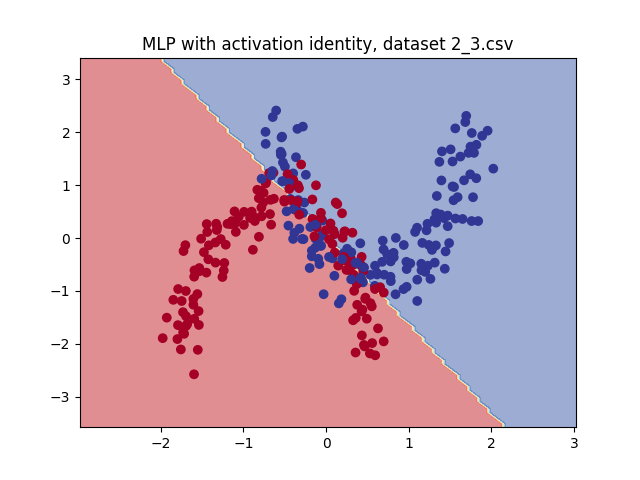
\includegraphics[width=\linewidth]{img/exp_1/mlp/2_3/identity/boundary.png}
        \caption{identity 2\_3}
    \end{subfigure}
    \hfill
    \begin{subfigure}[t]{\subfigwidth}
        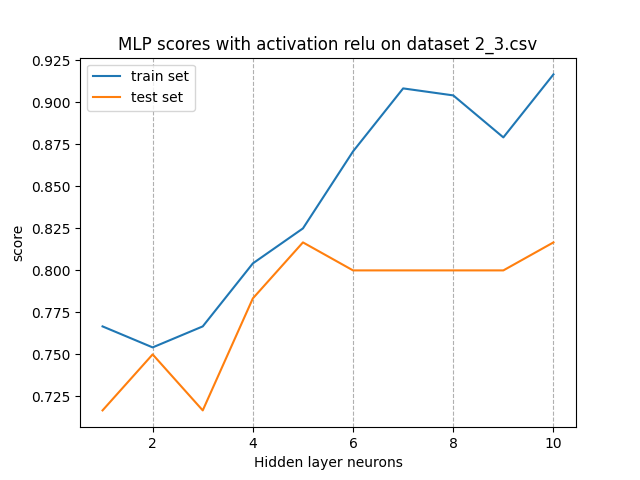
\includegraphics[width=\linewidth]{img/exp_1/mlp/2_3/relu/scores.png}
        \caption{ReLu 2\_3}
    \end{subfigure}
    \hfill
    \begin{subfigure}[t]{\subfigwidth}
        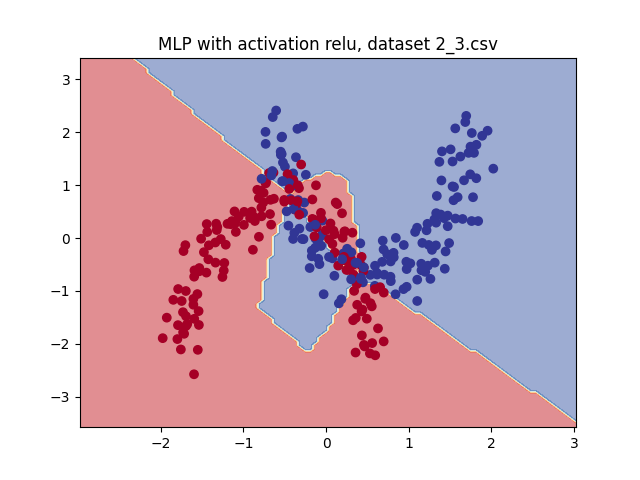
\includegraphics[width=\linewidth]{img/exp_1/mlp/2_3/relu/boundary.png}
        \caption{ReLu 2\_3}
    \end{subfigure}
    \caption{Eksperyment 1 --- Perceptron MLP}
\end{figure}

\begin{figure}[H]\centering
    \begin{subfigure}[t]{\subfigwidth}
        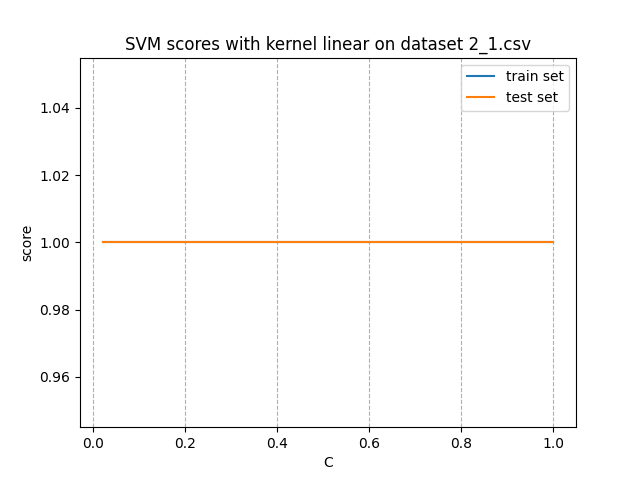
\includegraphics[width=\linewidth]{img/exp_1/svm/2_1/linear/scores.png}
        \caption{linear 2\_1}
    \end{subfigure}
    \hfill
    \begin{subfigure}[t]{\subfigwidth}
        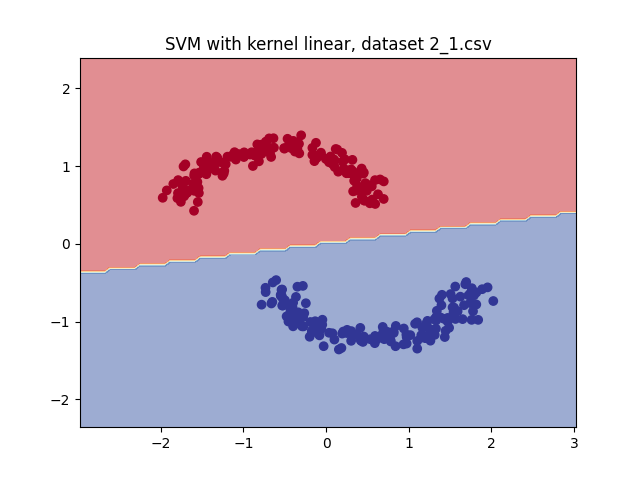
\includegraphics[width=\linewidth]{img/exp_1/svm/2_1/linear/boundary.png}
        \caption{linear 2\_1}
    \end{subfigure}
    \hfill
    \begin{subfigure}[t]{\subfigwidth}
        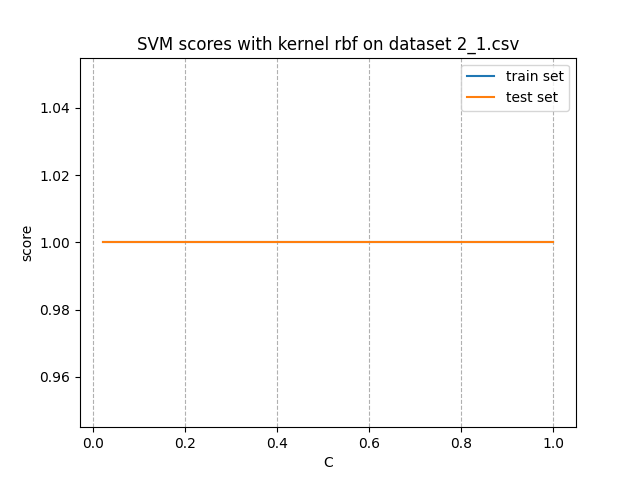
\includegraphics[width=\linewidth]{img/exp_1/svm/2_1/rbf/scores.png}
        \caption{rbf 2\_1}
    \end{subfigure}
    \hfill
    \begin{subfigure}[t]{\subfigwidth}
        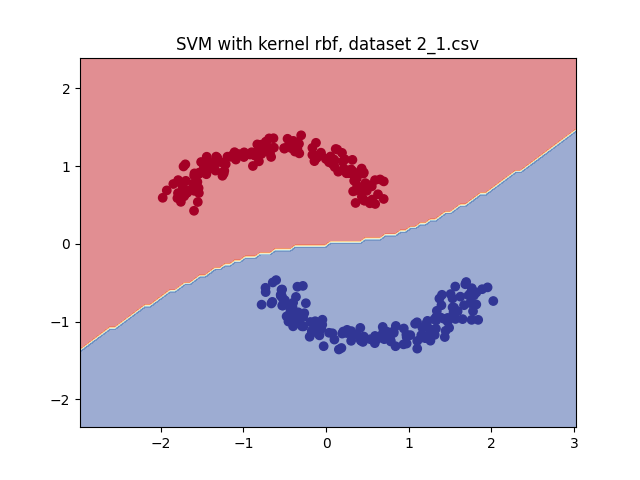
\includegraphics[width=\linewidth]{img/exp_1/svm/2_1/rbf/boundary.png}
        \caption{rbf 2\_1}
    \end{subfigure}
    \\
    \begin{subfigure}[t]{\subfigwidth}
        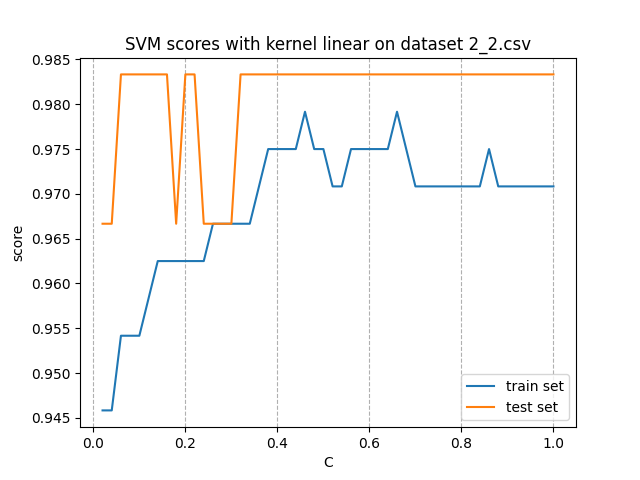
\includegraphics[width=\linewidth]{img/exp_1/svm/2_2/linear/scores.png}
        \caption{linear 2\_2}
    \end{subfigure}
    \hfill
    \begin{subfigure}[t]{\subfigwidth}
        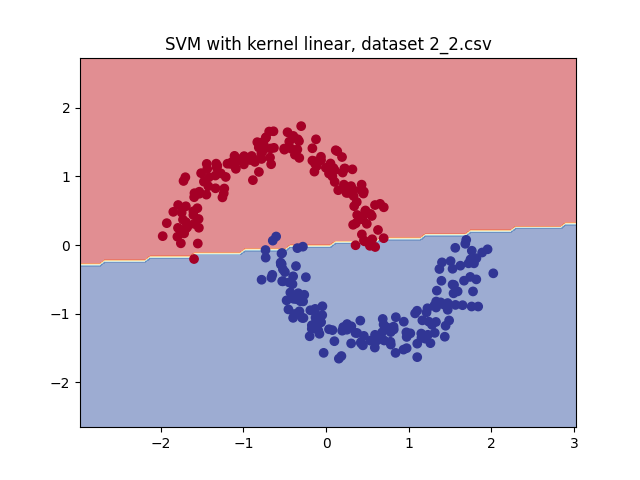
\includegraphics[width=\linewidth]{img/exp_1/svm/2_2/linear/boundary.png}
        \caption{linear 2\_2}
    \end{subfigure}
    \hfill
    \begin{subfigure}[t]{\subfigwidth}
        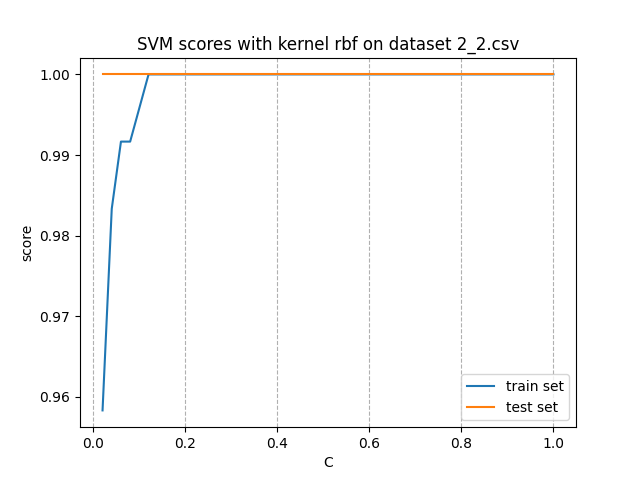
\includegraphics[width=\linewidth]{img/exp_1/svm/2_2/rbf/scores.png}
        \caption{rbf 2\_2}
    \end{subfigure}
    \hfill
    \begin{subfigure}[t]{\subfigwidth}
        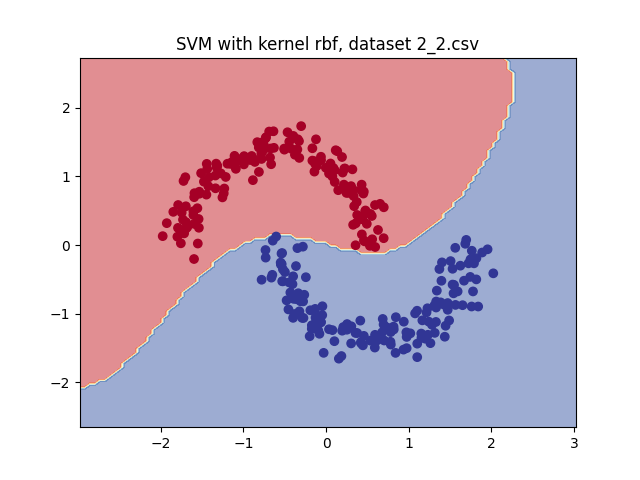
\includegraphics[width=\linewidth]{img/exp_1/svm/2_2/rbf/boundary.png}
        \caption{rbf 2\_2}
    \end{subfigure}
    \\
    \begin{subfigure}[t]{\subfigwidth}
        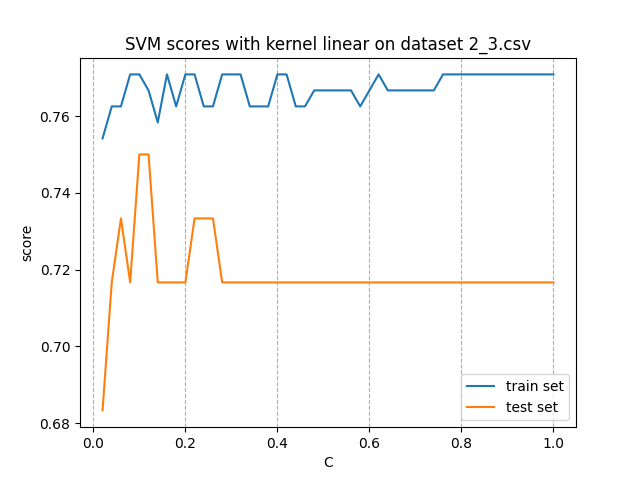
\includegraphics[width=\linewidth]{img/exp_1/svm/2_3/linear/scores.png}
        \caption{linear 2\_3}
    \end{subfigure}
    \hfill
    \begin{subfigure}[t]{\subfigwidth}
        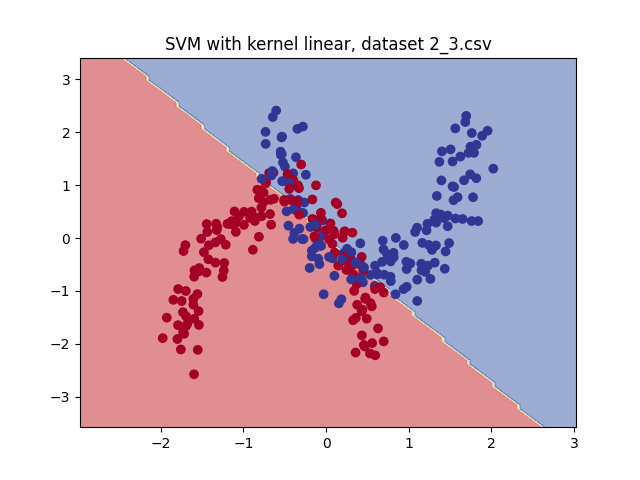
\includegraphics[width=\linewidth]{img/exp_1/svm/2_3/linear/boundary.png}
        \caption{linear 2\_3}
    \end{subfigure}
    \hfill
    \begin{subfigure}[t]{\subfigwidth}
        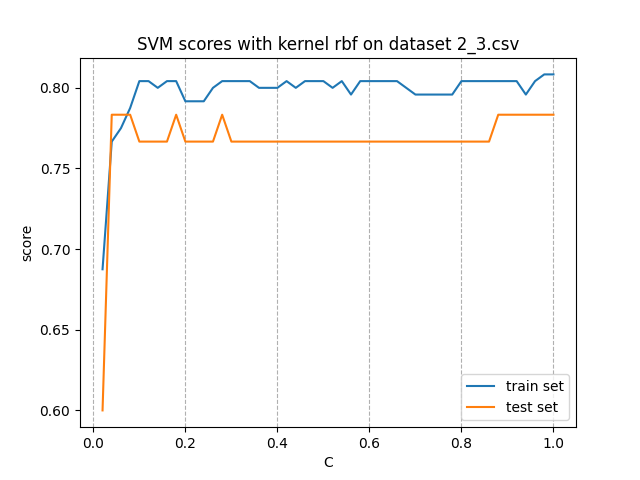
\includegraphics[width=\linewidth]{img/exp_1/svm/2_3/rbf/scores.png}
        \caption{rbf 2\_3}
    \end{subfigure}
    \hfill
    \begin{subfigure}[t]{\subfigwidth}
        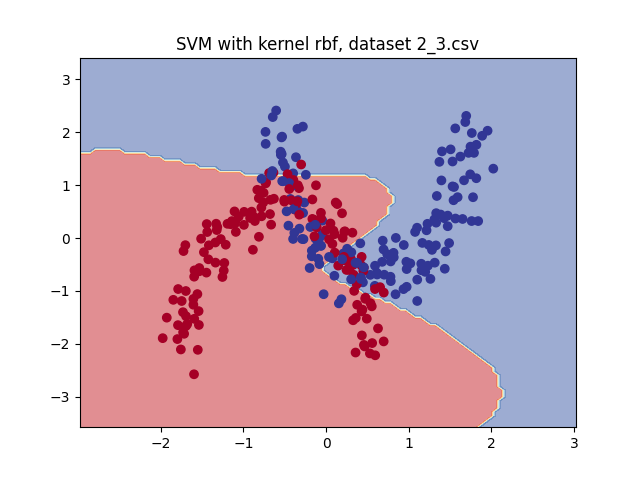
\includegraphics[width=\linewidth]{img/exp_1/svm/2_3/rbf/boundary.png}
        \caption{rbf 2\_3}
    \end{subfigure}
    \caption{Eksperyment 1 --- SVM}
\end{figure}

\clearpage

\renewcommand*{\subfigwidth}{0.16\textwidth}
\begin{figure}[H]\centering
    \begin{subfigure}[t]{\subfigwidth}
        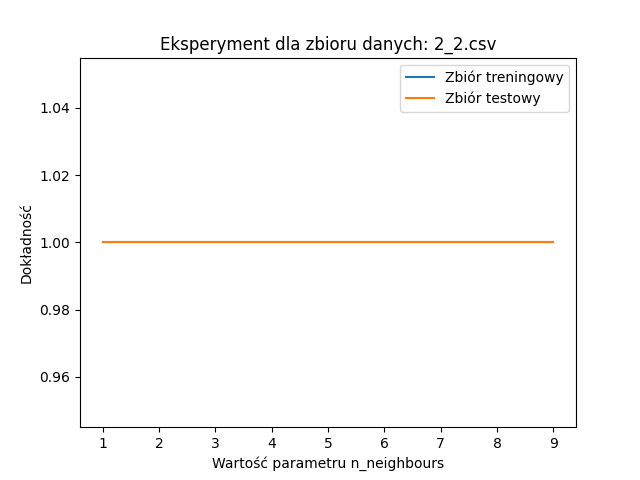
\includegraphics[width=\linewidth]{img/exp_2/knn/2_2/accuracy.png}
        \caption{Dokładność}
    \end{subfigure}
    \\
    \begin{subfigure}[t]{\subfigwidth}
        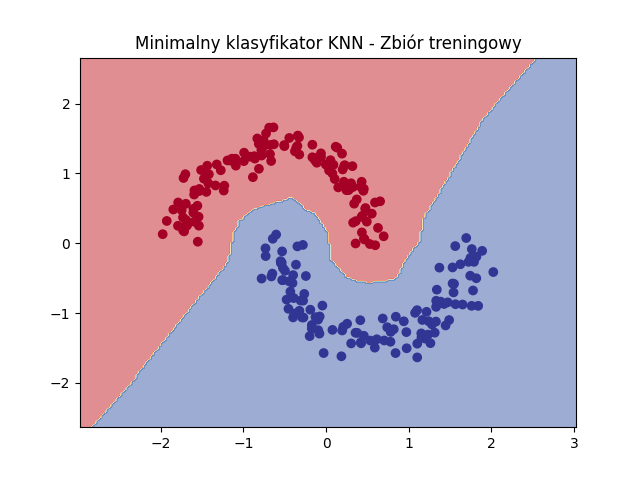
\includegraphics[width=\linewidth]{img/exp_2/knn/2_2/min/train_boundary.png}
        \caption{Min, train}
    \end{subfigure}
    \hfill
    \begin{subfigure}[t]{\subfigwidth}
        \includegraphics[width=\linewidth]{img/exp_2/knn/2_2/min/train_matrix.png}
        \caption{Min, train}
    \end{subfigure}
    \hfill
    \begin{subfigure}[t]{\subfigwidth}
        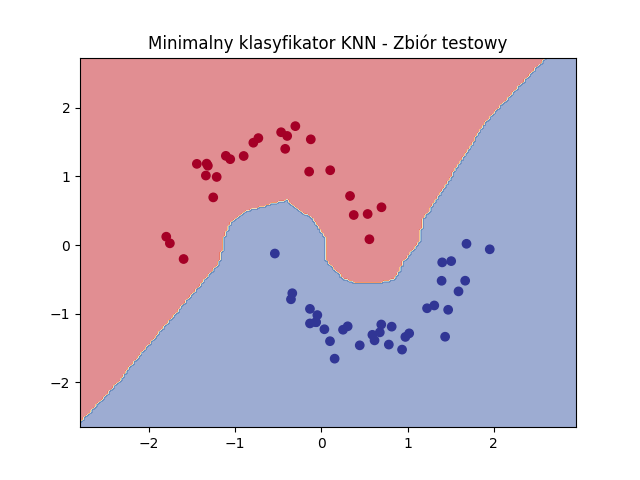
\includegraphics[width=\linewidth]{img/exp_2/knn/2_2/min/test_boundary.png}
        \caption{Min, test}
    \end{subfigure}
    \hfill
    \begin{subfigure}[t]{\subfigwidth}
        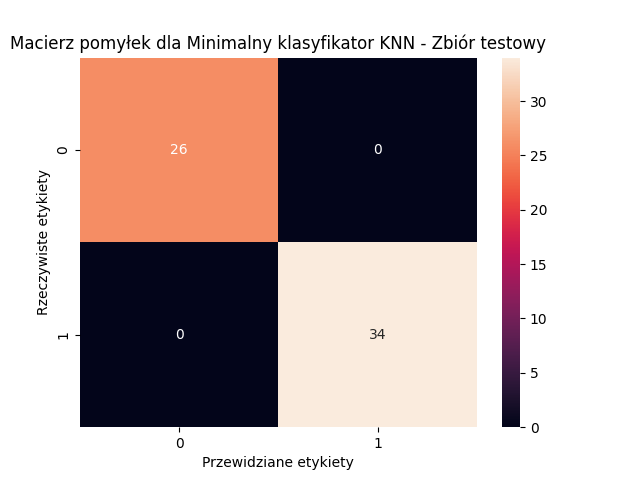
\includegraphics[width=\linewidth]{img/exp_2/knn/2_2/min/test_matrix.png}
        \caption{Min, test}
    \end{subfigure} 
    \\
    \begin{subfigure}[t]{\subfigwidth}
        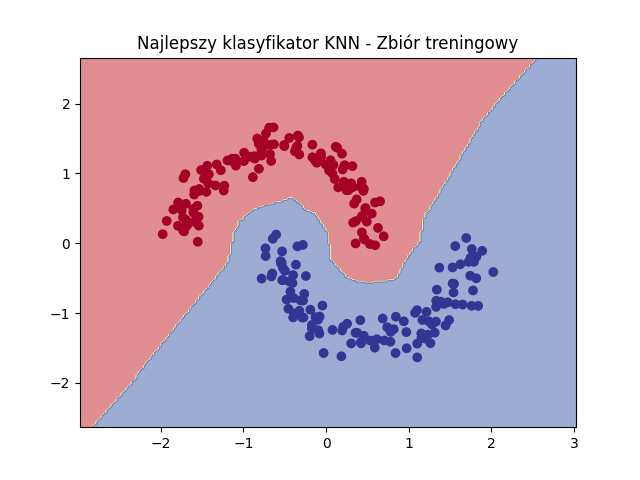
\includegraphics[width=\linewidth]{img/exp_2/knn/2_2/best/train_boundary.png}
        \caption{Best, train}
    \end{subfigure}
    \hfill
    \begin{subfigure}[t]{\subfigwidth}
        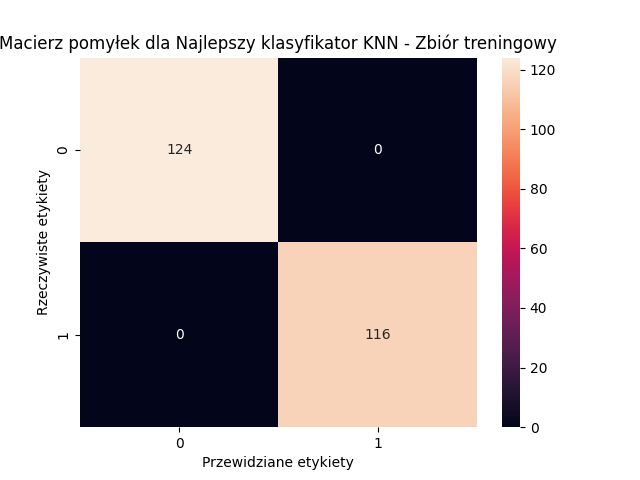
\includegraphics[width=\linewidth]{img/exp_2/knn/2_2/best/train_matrix.png}
        \caption{Best, train}
    \end{subfigure}
    \hfill
    \begin{subfigure}[t]{\subfigwidth}
        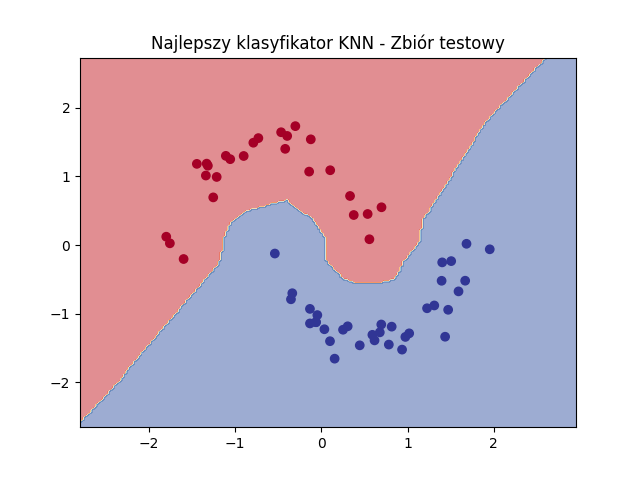
\includegraphics[width=\linewidth]{img/exp_2/knn/2_2/best/test_boundary.png}
        \caption{Best, test}
    \end{subfigure}
    \hfill
    \begin{subfigure}[t]{\subfigwidth}
        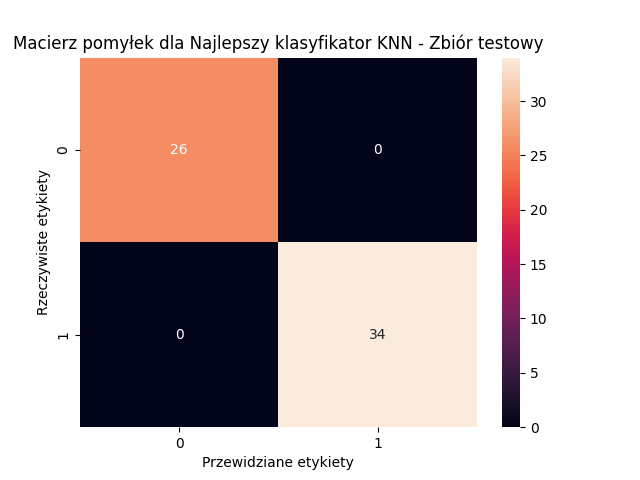
\includegraphics[width=\linewidth]{img/exp_2/knn/2_2/best/test_matrix.png}
        \caption{Best, test}
    \end{subfigure} 
    \\
    \begin{subfigure}[t]{\subfigwidth}
        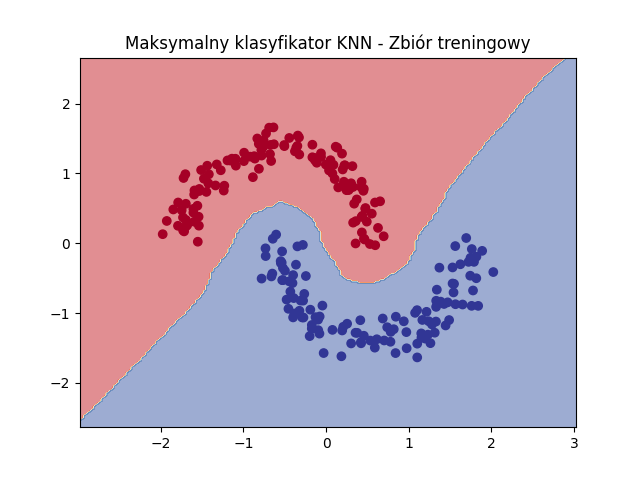
\includegraphics[width=\linewidth]{img/exp_2/knn/2_2/max/train_boundary.png}
        \caption{Max, train}
    \end{subfigure}
    \hfill
    \begin{subfigure}[t]{\subfigwidth}
        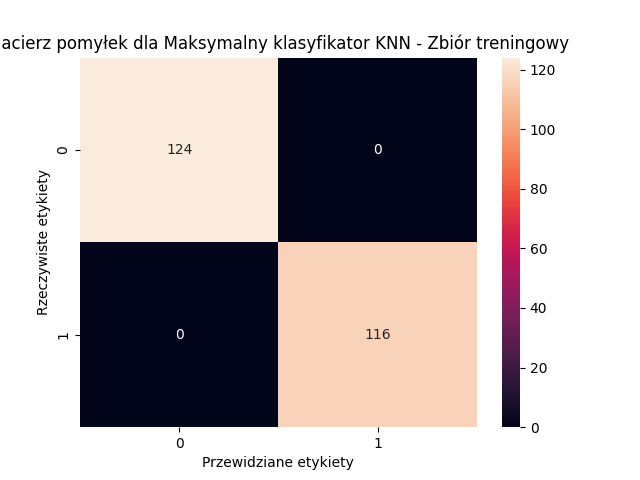
\includegraphics[width=\linewidth]{img/exp_2/knn/2_2/max/train_matrix.png}
        \caption{Max, train}
    \end{subfigure}
    \hfill
    \begin{subfigure}[t]{\subfigwidth}
        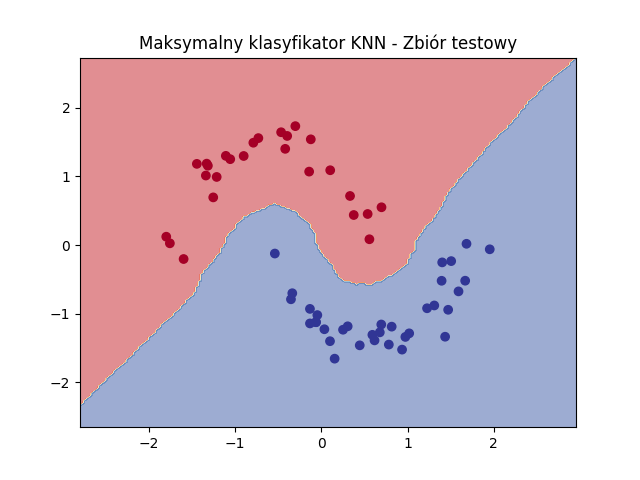
\includegraphics[width=\linewidth]{img/exp_2/knn/2_2/max/test_boundary.png}
        \caption{Max, test}
    \end{subfigure}
    \hfill
    \begin{subfigure}[t]{\subfigwidth}
        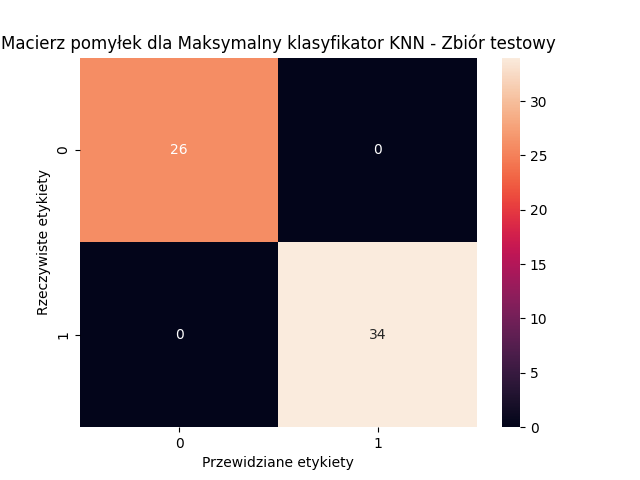
\includegraphics[width=\linewidth]{img/exp_2/knn/2_2/max/test_matrix.png}
        \caption{Max, test}
    \end{subfigure} 
    
    \caption{Eksperyment 2 --- KNN na zbiorze 2\_2}
\end{figure}

\begin{figure}[H]\centering
    \begin{subfigure}[t]{\subfigwidth}
        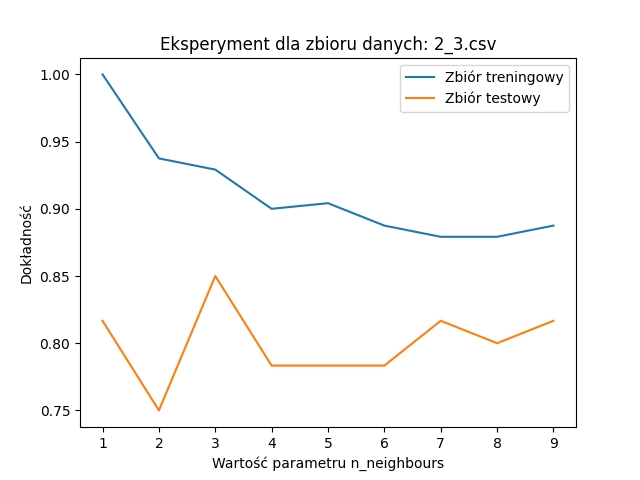
\includegraphics[width=\linewidth]{img/exp_2/knn/2_3/accuracy.png}
        \caption{Dokładność}
    \end{subfigure}
    \\
    \begin{subfigure}[t]{\subfigwidth}
        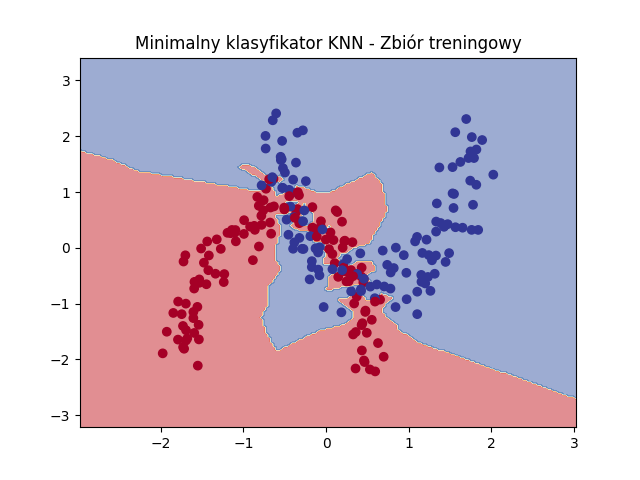
\includegraphics[width=\linewidth]{img/exp_2/knn/2_3/min/train_boundary.png}
        \caption{Min, train}
    \end{subfigure}
    \hfill
    \begin{subfigure}[t]{\subfigwidth}
        \includegraphics[width=\linewidth]{img/exp_2/knn/2_3/min/train_matrix.png}
        \caption{Min, train}
    \end{subfigure}
    \hfill
    \begin{subfigure}[t]{\subfigwidth}
        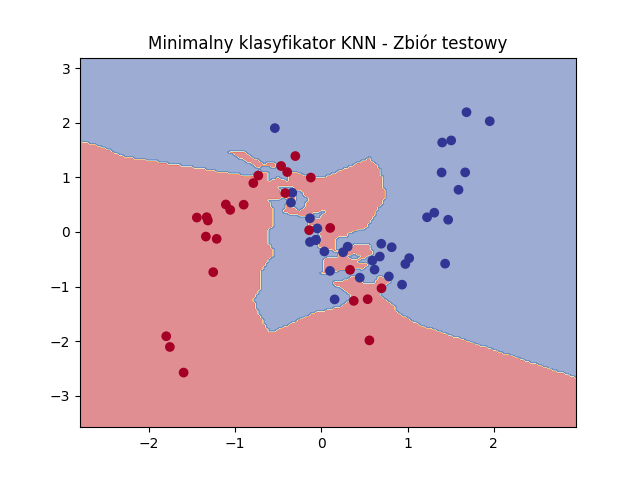
\includegraphics[width=\linewidth]{img/exp_2/knn/2_3/min/test_boundary.png}
        \caption{Min, test}
    \end{subfigure}
    \hfill
    \begin{subfigure}[t]{\subfigwidth}
        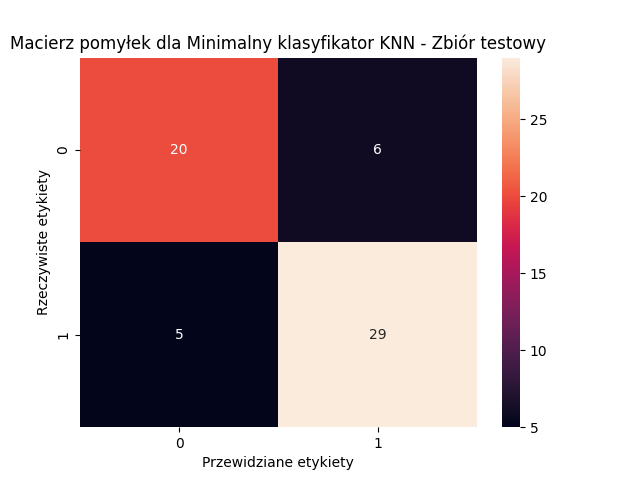
\includegraphics[width=\linewidth]{img/exp_2/knn/2_3/min/test_matrix.png}
        \caption{Min, test}
    \end{subfigure} 
    \\
    \begin{subfigure}[t]{\subfigwidth}
        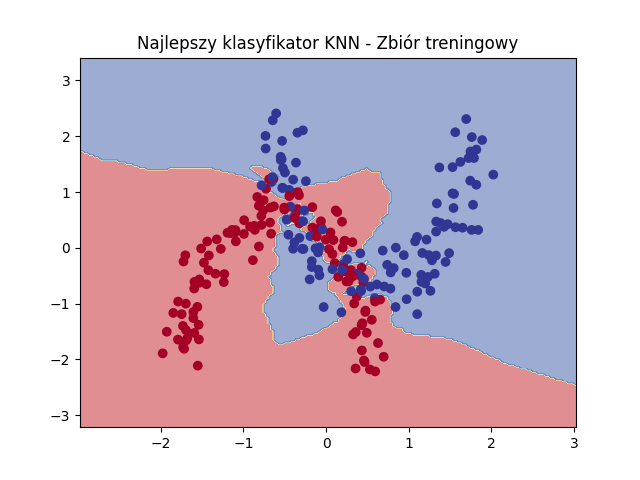
\includegraphics[width=\linewidth]{img/exp_2/knn/2_3/best/train_boundary.png}
        \caption{Best, train}
    \end{subfigure}
    \hfill
    \begin{subfigure}[t]{\subfigwidth}
        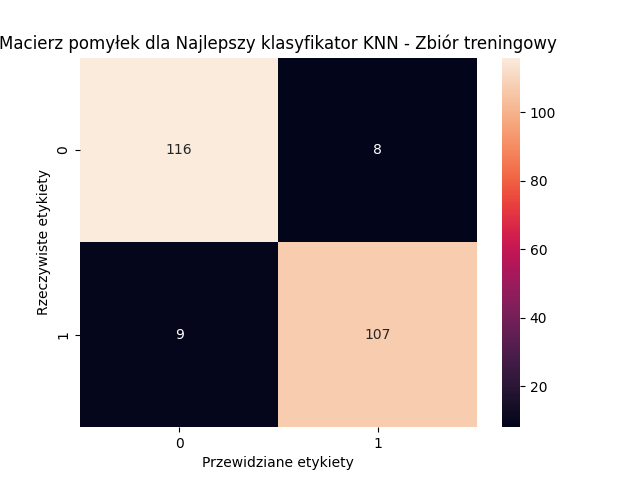
\includegraphics[width=\linewidth]{img/exp_2/knn/2_3/best/train_matrix.png}
        \caption{Best, train}
    \end{subfigure}
    \hfill
    \begin{subfigure}[t]{\subfigwidth}
        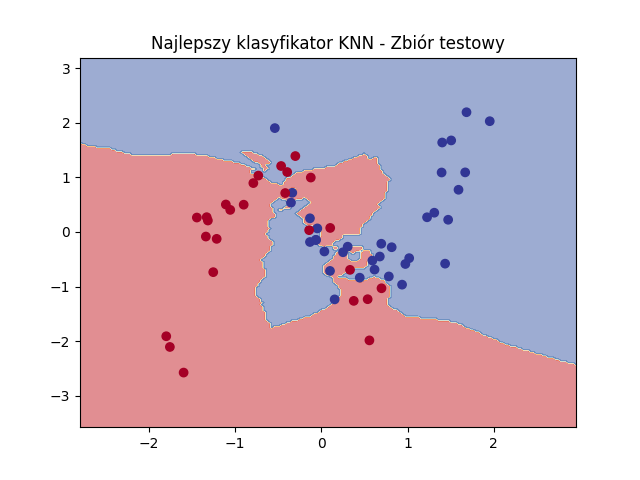
\includegraphics[width=\linewidth]{img/exp_2/knn/2_3/best/test_boundary.png}
        \caption{Best, test}
    \end{subfigure}
    \hfill
    \begin{subfigure}[t]{\subfigwidth}
        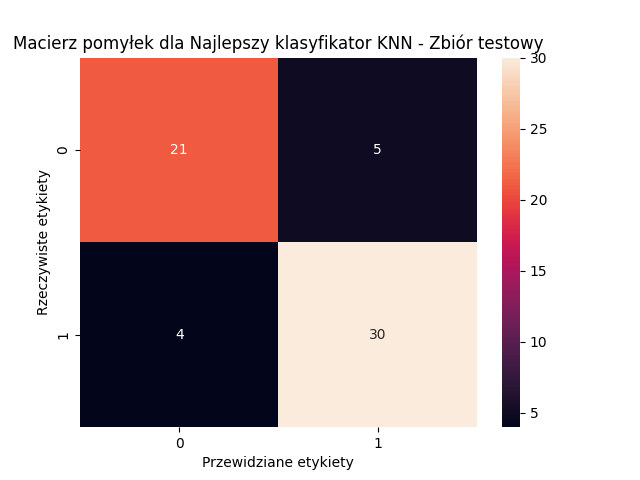
\includegraphics[width=\linewidth]{img/exp_2/knn/2_3/best/test_matrix.png}
        \caption{Best, test}
    \end{subfigure} 
    \\
    \begin{subfigure}[t]{\subfigwidth}
        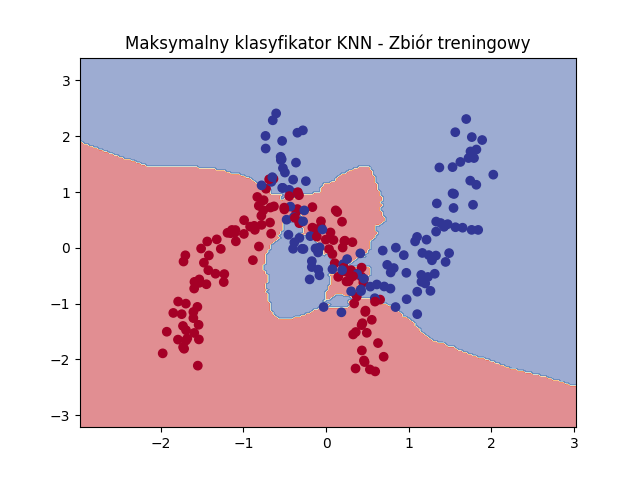
\includegraphics[width=\linewidth]{img/exp_2/knn/2_3/max/train_boundary.png}
        \caption{Max, train}
    \end{subfigure}
    \hfill
    \begin{subfigure}[t]{\subfigwidth}
        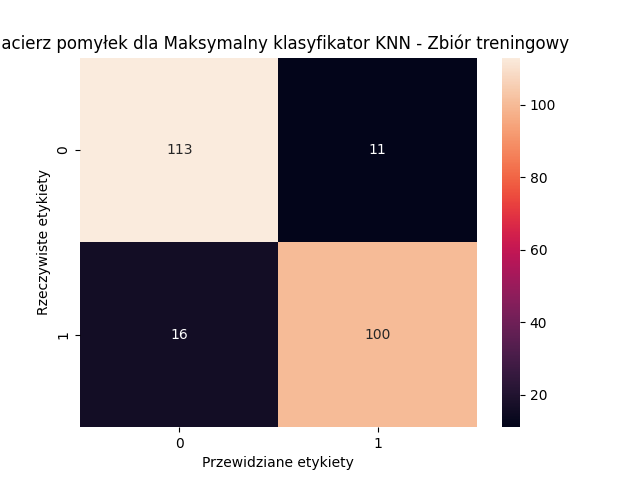
\includegraphics[width=\linewidth]{img/exp_2/knn/2_3/max/train_matrix.png}
        \caption{Max, train}
    \end{subfigure}
    \hfill
    \begin{subfigure}[t]{\subfigwidth}
        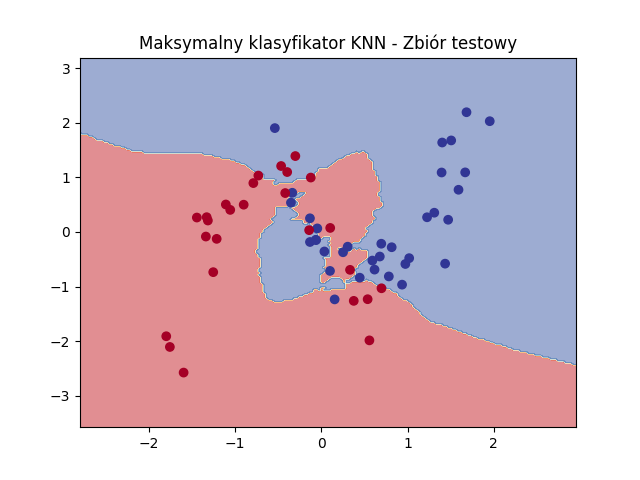
\includegraphics[width=\linewidth]{img/exp_2/knn/2_3/max/test_boundary.png}
        \caption{Max, test}
    \end{subfigure}
    \hfill
    \begin{subfigure}[t]{\subfigwidth}
        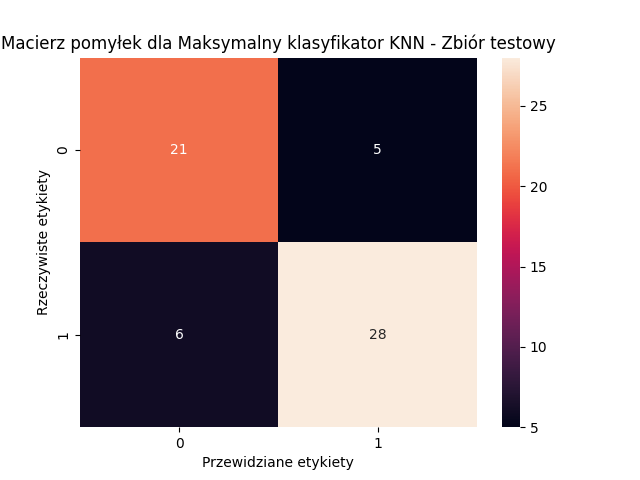
\includegraphics[width=\linewidth]{img/exp_2/knn/2_3/max/test_matrix.png}
        \caption{Max, test}
    \end{subfigure} 
    
    \caption{Eksperyment 2 --- KNN na zbiorze 2\_3}
\end{figure}

\clearpage

\begin{figure}[H]\centering
    \begin{subfigure}[t]{\subfigwidth}
        \includegraphics[width=\linewidth]{img/exp_2/svm/2_2/accuracy.png}
        \caption{Dokładność}
    \end{subfigure}
    \\
    \begin{subfigure}[t]{\subfigwidth}
        \includegraphics[width=\linewidth]{img/exp_2/svm/2_2/min/train_boundary.png}
        \caption{Min, train}
    \end{subfigure}
    \hfill
    \begin{subfigure}[t]{\subfigwidth}
        \includegraphics[width=\linewidth]{img/exp_2/svm/2_2/min/train_matrix.png}
        \caption{Min, train}
    \end{subfigure}
    \hfill
    \begin{subfigure}[t]{\subfigwidth}
        \includegraphics[width=\linewidth]{img/exp_2/svm/2_2/min/test_boundary.png}
        \caption{Min, test}
    \end{subfigure}
    \hfill
    \begin{subfigure}[t]{\subfigwidth}
        \includegraphics[width=\linewidth]{img/exp_2/svm/2_2/min/test_matrix.png}
        \caption{Min, test}
    \end{subfigure} 
    \\
    \begin{subfigure}[t]{\subfigwidth}
        \includegraphics[width=\linewidth]{img/exp_2/svm/2_2/best/train_boundary.png}
        \caption{Best, train}
    \end{subfigure}
    \hfill
    \begin{subfigure}[t]{\subfigwidth}
        \includegraphics[width=\linewidth]{img/exp_2/svm/2_2/best/train_matrix.png}
        \caption{Best, train}
    \end{subfigure}
    \hfill
    \begin{subfigure}[t]{\subfigwidth}
        \includegraphics[width=\linewidth]{img/exp_2/svm/2_2/best/test_boundary.png}
        \caption{Best, test}
    \end{subfigure}
    \hfill
    \begin{subfigure}[t]{\subfigwidth}
        \includegraphics[width=\linewidth]{img/exp_2/svm/2_2/best/test_matrix.png}
        \caption{Best, test}
    \end{subfigure} 
    \\
    \begin{subfigure}[t]{\subfigwidth}
        \includegraphics[width=\linewidth]{img/exp_2/svm/2_2/max/train_boundary.png}
        \caption{Max, train}
    \end{subfigure}
    \hfill
    \begin{subfigure}[t]{\subfigwidth}
        \includegraphics[width=\linewidth]{img/exp_2/svm/2_2/max/train_matrix.png}
        \caption{Max, train}
    \end{subfigure}
    \hfill
    \begin{subfigure}[t]{\subfigwidth}
        \includegraphics[width=\linewidth]{img/exp_2/svm/2_2/max/test_boundary.png}
        \caption{Max, test}
    \end{subfigure}
    \hfill
    \begin{subfigure}[t]{\subfigwidth}
        \includegraphics[width=\linewidth]{img/exp_2/svm/2_2/max/test_matrix.png}
        \caption{Max, test}
    \end{subfigure} 
    
    \caption{Eksperyment 2 --- SVM na zbiorze 2\_2}
\end{figure}

\begin{figure}[H]\centering
    \begin{subfigure}[t]{\subfigwidth}
        \includegraphics[width=\linewidth]{img/exp_2/svm/2_3/accuracy.png}
        \caption{Dokładność}
    \end{subfigure}
    \\
    \begin{subfigure}[t]{\subfigwidth}
        \includegraphics[width=\linewidth]{img/exp_2/svm/2_3/min/train_boundary.png}
        \caption{Min, train}
    \end{subfigure}
    \hfill
    \begin{subfigure}[t]{\subfigwidth}
        \includegraphics[width=\linewidth]{img/exp_2/svm/2_3/min/train_matrix.png}
        \caption{Min, train}
    \end{subfigure}
    \hfill
    \begin{subfigure}[t]{\subfigwidth}
        \includegraphics[width=\linewidth]{img/exp_2/svm/2_3/min/test_boundary.png}
        \caption{Min, test}
    \end{subfigure}
    \hfill
    \begin{subfigure}[t]{\subfigwidth}
        \includegraphics[width=\linewidth]{img/exp_2/svm/2_3/min/test_matrix.png}
        \caption{Min, test}
    \end{subfigure} 
    \\
    \begin{subfigure}[t]{\subfigwidth}
        \includegraphics[width=\linewidth]{img/exp_2/svm/2_3/best/train_boundary.png}
        \caption{Best, train}
    \end{subfigure}
    \hfill
    \begin{subfigure}[t]{\subfigwidth}
        \includegraphics[width=\linewidth]{img/exp_2/svm/2_3/best/train_matrix.png}
        \caption{Best, train}
    \end{subfigure}
    \hfill
    \begin{subfigure}[t]{\subfigwidth}
        \includegraphics[width=\linewidth]{img/exp_2/svm/2_3/best/test_boundary.png}
        \caption{Best, test}
    \end{subfigure}
    \hfill
    \begin{subfigure}[t]{\subfigwidth}
        \includegraphics[width=\linewidth]{img/exp_2/svm/2_3/best/test_matrix.png}
        \caption{Best, test}
    \end{subfigure} 
    \\
    \begin{subfigure}[t]{\subfigwidth}
        \includegraphics[width=\linewidth]{img/exp_2/svm/2_3/max/train_boundary.png}
        \caption{Max, train}
    \end{subfigure}
    \hfill
    \begin{subfigure}[t]{\subfigwidth}
        \includegraphics[width=\linewidth]{img/exp_2/svm/2_3/max/train_matrix.png}
        \caption{Max, train}
    \end{subfigure}
    \hfill
    \begin{subfigure}[t]{\subfigwidth}
        \includegraphics[width=\linewidth]{img/exp_2/svm/2_3/max/test_boundary.png}
        \caption{Max, test}
    \end{subfigure}
    \hfill
    \begin{subfigure}[t]{\subfigwidth}
        \includegraphics[width=\linewidth]{img/exp_2/svm/2_3/max/test_matrix.png}
        \caption{Max, test}
    \end{subfigure} 
    
    \caption{Eksperyment 2 --- SVM na zbiorze 2\_3}
\end{figure}

\clearpage

\begin{figure}[H]\centering
    \begin{subfigure}[t]{\subfigwidth}
        \includegraphics[width=\linewidth]{img/exp_2/mlp/2_2/accuracy.png}
        \caption{Dokładność}
    \end{subfigure}
    \\
    \begin{subfigure}[t]{\subfigwidth}
        \includegraphics[width=\linewidth]{img/exp_2/mlp/2_2/min/train_boundary.png}
        \caption{Min, train}
    \end{subfigure}
    \hfill
    \begin{subfigure}[t]{\subfigwidth}
        \includegraphics[width=\linewidth]{img/exp_2/mlp/2_2/min/train_matrix.png}
        \caption{Min, train}
    \end{subfigure}
    \hfill
    \begin{subfigure}[t]{\subfigwidth}
        \includegraphics[width=\linewidth]{img/exp_2/mlp/2_2/min/test_boundary.png}
        \caption{Min, test}
    \end{subfigure}
    \hfill
    \begin{subfigure}[t]{\subfigwidth}
        \includegraphics[width=\linewidth]{img/exp_2/mlp/2_2/min/test_matrix.png}
        \caption{Min, test}
    \end{subfigure} 
    \\
    \begin{subfigure}[t]{\subfigwidth}
        \includegraphics[width=\linewidth]{img/exp_2/mlp/2_2/best/train_boundary.png}
        \caption{Best, train}
    \end{subfigure}
    \hfill
    \begin{subfigure}[t]{\subfigwidth}
        \includegraphics[width=\linewidth]{img/exp_2/mlp/2_2/best/train_matrix.png}
        \caption{Best, train}
    \end{subfigure}
    \hfill
    \begin{subfigure}[t]{\subfigwidth}
        \includegraphics[width=\linewidth]{img/exp_2/mlp/2_2/best/test_boundary.png}
        \caption{Best, test}
    \end{subfigure}
    \hfill
    \begin{subfigure}[t]{\subfigwidth}
        \includegraphics[width=\linewidth]{img/exp_2/mlp/2_2/best/test_matrix.png}
        \caption{Best, test}
    \end{subfigure} 
    \\
    \begin{subfigure}[t]{\subfigwidth}
        \includegraphics[width=\linewidth]{img/exp_2/mlp/2_2/max/train_boundary.png}
        \caption{Max, train}
    \end{subfigure}
    \hfill
    \begin{subfigure}[t]{\subfigwidth}
        \includegraphics[width=\linewidth]{img/exp_2/mlp/2_2/max/train_matrix.png}
        \caption{Max, train}
    \end{subfigure}
    \hfill
    \begin{subfigure}[t]{\subfigwidth}
        \includegraphics[width=\linewidth]{img/exp_2/mlp/2_2/max/test_boundary.png}
        \caption{Max, test}
    \end{subfigure}
    \hfill
    \begin{subfigure}[t]{\subfigwidth}
        \includegraphics[width=\linewidth]{img/exp_2/mlp/2_2/max/test_matrix.png}
        \caption{Max, test}
    \end{subfigure} 
    
    \caption{Eksperyment 2 --- MLP na zbiorze 2\_2}
\end{figure}

\begin{figure}[H]\centering
    \begin{subfigure}[t]{\subfigwidth}
        \includegraphics[width=\linewidth]{img/exp_2/mlp/2_3/accuracy.png}
        \caption{Dokładność}
    \end{subfigure}
    \\
    \begin{subfigure}[t]{\subfigwidth}
        \includegraphics[width=\linewidth]{img/exp_2/mlp/2_3/min/train_boundary.png}
        \caption{Min, train}
    \end{subfigure}
    \hfill
    \begin{subfigure}[t]{\subfigwidth}
        \includegraphics[width=\linewidth]{img/exp_2/mlp/2_3/min/train_matrix.png}
        \caption{Min, train}
    \end{subfigure}
    \hfill
    \begin{subfigure}[t]{\subfigwidth}
        \includegraphics[width=\linewidth]{img/exp_2/mlp/2_3/min/test_boundary.png}
        \caption{Min, test}
    \end{subfigure}
    \hfill
    \begin{subfigure}[t]{\subfigwidth}
        \includegraphics[width=\linewidth]{img/exp_2/mlp/2_3/min/test_matrix.png}
        \caption{Min, test}
    \end{subfigure} 
    \\
    \begin{subfigure}[t]{\subfigwidth}
        \includegraphics[width=\linewidth]{img/exp_2/mlp/2_3/best/train_boundary.png}
        \caption{Best, train}
    \end{subfigure}
    \hfill
    \begin{subfigure}[t]{\subfigwidth}
        \includegraphics[width=\linewidth]{img/exp_2/mlp/2_3/best/train_matrix.png}
        \caption{Best, train}
    \end{subfigure}
    \hfill
    \begin{subfigure}[t]{\subfigwidth}
        \includegraphics[width=\linewidth]{img/exp_2/mlp/2_3/best/test_boundary.png}
        \caption{Best, test}
    \end{subfigure}
    \hfill
    \begin{subfigure}[t]{\subfigwidth}
        \includegraphics[width=\linewidth]{img/exp_2/mlp/2_3/best/test_matrix.png}
        \caption{Best, test}
    \end{subfigure} 
    \\
    \begin{subfigure}[t]{\subfigwidth}
        \includegraphics[width=\linewidth]{img/exp_2/mlp/2_3/max/train_boundary.png}
        \caption{Max, train}
    \end{subfigure}
    \hfill
    \begin{subfigure}[t]{\subfigwidth}
        \includegraphics[width=\linewidth]{img/exp_2/mlp/2_3/max/train_matrix.png}
        \caption{Max, train}
    \end{subfigure}
    \hfill
    \begin{subfigure}[t]{\subfigwidth}
        \includegraphics[width=\linewidth]{img/exp_2/mlp/2_3/max/test_boundary.png}
        \caption{Max, test}
    \end{subfigure}
    \hfill
    \begin{subfigure}[t]{\subfigwidth}
        \includegraphics[width=\linewidth]{img/exp_2/mlp/2_3/max/test_matrix.png}
        \caption{Max, test}
    \end{subfigure} 
    
    \caption{Eksperyment 2 --- MLP na zbiorze 2\_3}
\end{figure}

\clearpage
% 5 strona --- Wyniki trzeciego eksperymentu dla dwóch sztucznie wygenerowanych zbiorów danych 2\_2 i 2\_3 oraz metody K-NN. Dla każdego zbioru należy pokazać wykres obrazujący zmianę wartości accuracy na zbiorach treningowym i testowym przy zmieniającym się parametrze n\_neighbours oraz wizualizacje przebiegu granicy decyzyjnej na zbiorach treningowym i testowym dla: najmniejszej, najlepszej (wartość accuracy na zbiorze testowym) i największej wartości tego parametru. Dodatkowo przy każdej wizualizacji należy pokazać jak wygląda macierz pomyłek.
\begin{figure}[H]\centering
    \begin{subfigure}[t]{\subfigwidth}
        \includegraphics[width=\linewidth]{img/exp_3/knn/2_2/accuracy.png}
        \caption{Dokładność}
    \end{subfigure}
    \\
    \begin{subfigure}[t]{\subfigwidth}
        \includegraphics[width=\linewidth]{img/exp_3/knn/2_2/min/train_boundary.png}
        \caption{Min, train}
    \end{subfigure}
    \hfill
    \begin{subfigure}[t]{\subfigwidth}
        \includegraphics[width=\linewidth]{img/exp_3/knn/2_2/min/train_matrix.png}
        \caption{Min, train}
    \end{subfigure}
    \hfill
    \begin{subfigure}[t]{\subfigwidth}
        \includegraphics[width=\linewidth]{img/exp_3/knn/2_2/min/test_boundary.png}
        \caption{Min, test}
    \end{subfigure}
    \hfill
    \begin{subfigure}[t]{\subfigwidth}
        \includegraphics[width=\linewidth]{img/exp_3/knn/2_2/min/test_matrix.png}
        \caption{Min, test}
    \end{subfigure} 
    \\
    \begin{subfigure}[t]{\subfigwidth}
        \includegraphics[width=\linewidth]{img/exp_3/knn/2_2/best/train_boundary.png}
        \caption{Best, train}
    \end{subfigure}
    \hfill
    \begin{subfigure}[t]{\subfigwidth}
        \includegraphics[width=\linewidth]{img/exp_3/knn/2_2/best/train_matrix.png}
        \caption{Best, train}
    \end{subfigure}
    \hfill
    \begin{subfigure}[t]{\subfigwidth}
        \includegraphics[width=\linewidth]{img/exp_3/knn/2_2/best/test_boundary.png}
        \caption{Best, test}
    \end{subfigure}
    \hfill
    \begin{subfigure}[t]{\subfigwidth}
        \includegraphics[width=\linewidth]{img/exp_3/knn/2_2/best/test_matrix.png}
        \caption{Best, test}
    \end{subfigure} 
    \\
    \begin{subfigure}[t]{\subfigwidth}
        \includegraphics[width=\linewidth]{img/exp_3/knn/2_2/max/train_boundary.png}
        \caption{Max, train}
    \end{subfigure}
    \hfill
    \begin{subfigure}[t]{\subfigwidth}
        \includegraphics[width=\linewidth]{img/exp_3/knn/2_2/max/train_matrix.png}
        \caption{Max, train}
    \end{subfigure}
    \hfill
    \begin{subfigure}[t]{\subfigwidth}
        \includegraphics[width=\linewidth]{img/exp_3/knn/2_2/max/test_boundary.png}
        \caption{Max, test}
    \end{subfigure}
    \hfill
    \begin{subfigure}[t]{\subfigwidth}
        \includegraphics[width=\linewidth]{img/exp_3/knn/2_2/max/test_matrix.png}
        \caption{Max, test}
    \end{subfigure} 
    
    \caption{Eksperyment 3 --- KNN na zbiorze 2\_2}
\end{figure}

\begin{figure}[H]\centering
    \begin{subfigure}[t]{\subfigwidth}
        \includegraphics[width=\linewidth]{img/exp_3/knn/2_3/accuracy.png}
        \caption{Dokładność}
    \end{subfigure}
    \\
    \begin{subfigure}[t]{\subfigwidth}
        \includegraphics[width=\linewidth]{img/exp_3/knn/2_3/min/train_boundary.png}
        \caption{Min, train}
    \end{subfigure}
    \hfill
    \begin{subfigure}[t]{\subfigwidth}
        \includegraphics[width=\linewidth]{img/exp_3/knn/2_3/min/train_matrix.png}
        \caption{Min, train}
    \end{subfigure}
    \hfill
    \begin{subfigure}[t]{\subfigwidth}
        \includegraphics[width=\linewidth]{img/exp_3/knn/2_3/min/test_boundary.png}
        \caption{Min, test}
    \end{subfigure}
    \hfill
    \begin{subfigure}[t]{\subfigwidth}
        \includegraphics[width=\linewidth]{img/exp_3/knn/2_3/min/test_matrix.png}
        \caption{Min, test}
    \end{subfigure} 
    \\
    \begin{subfigure}[t]{\subfigwidth}
        \includegraphics[width=\linewidth]{img/exp_3/knn/2_3/best/train_boundary.png}
        \caption{Best, train}
    \end{subfigure}
    \hfill
    \begin{subfigure}[t]{\subfigwidth}
        \includegraphics[width=\linewidth]{img/exp_3/knn/2_3/best/train_matrix.png}
        \caption{Best, train}
    \end{subfigure}
    \hfill
    \begin{subfigure}[t]{\subfigwidth}
        \includegraphics[width=\linewidth]{img/exp_3/knn/2_3/best/test_boundary.png}
        \caption{Best, test}
    \end{subfigure}
    \hfill
    \begin{subfigure}[t]{\subfigwidth}
        \includegraphics[width=\linewidth]{img/exp_3/knn/2_3/best/test_matrix.png}
        \caption{Best, test}
    \end{subfigure} 
    \\
    \begin{subfigure}[t]{\subfigwidth}
        \includegraphics[width=\linewidth]{img/exp_3/knn/2_3/max/train_boundary.png}
        \caption{Max, train}
    \end{subfigure}
    \hfill
    \begin{subfigure}[t]{\subfigwidth}
        \includegraphics[width=\linewidth]{img/exp_3/knn/2_3/max/train_matrix.png}
        \caption{Max, train}
    \end{subfigure}
    \hfill
    \begin{subfigure}[t]{\subfigwidth}
        \includegraphics[width=\linewidth]{img/exp_3/knn/2_3/max/test_boundary.png}
        \caption{Max, test}
    \end{subfigure}
    \hfill
    \begin{subfigure}[t]{\subfigwidth}
        \includegraphics[width=\linewidth]{img/exp_3/knn/2_3/max/test_matrix.png}
        \caption{Max, test}
    \end{subfigure} 
    
    \caption{Eksperyment 3 --- KNN na zbiorze 2\_3}
\end{figure}

\clearpage

% 6 strona --- Wyniki trzeciego eksperymentu dla dwóch sztucznie wygenerowanych zbiorów danych 2\_2 i 2\_3 oraz metody SVM. Dla każdego zbioru należy pokazać wykres obrazujący zmianę wartości accuracy na zbiorach treningowym i testowym przy zmieniającym się parametrze C oraz wizualizacje przebiegu granicy decyzyjnej na zbiorach treningowym i testowym dla: najmniejszej, najlepszej (wartość accuracy na zbiorze testowym) i największej wartości tego parametru. Dodatkowo przy każdej wizualizacji należy pokazać jak wygląda macierz pomyłek. Wartości parametru C powinny się zmieniać wykładniczo, a na wykresie dobrze jest zastosować skalę logarytmiczną.
\begin{figure}[H]\centering
    \begin{subfigure}[t]{\subfigwidth}
        \includegraphics[width=\linewidth]{img/exp_3/svm/2_2/accuracy.png}
        \caption{Dokładność}
    \end{subfigure}
    \\
    \begin{subfigure}[t]{\subfigwidth}
        \includegraphics[width=\linewidth]{img/exp_3/svm/2_2/min/train_boundary.png}
        \caption{Min, train}
    \end{subfigure}
    \hfill
    \begin{subfigure}[t]{\subfigwidth}
        \includegraphics[width=\linewidth]{img/exp_3/svm/2_2/min/train_matrix.png}
        \caption{Min, train}
    \end{subfigure}
    \hfill
    \begin{subfigure}[t]{\subfigwidth}
        \includegraphics[width=\linewidth]{img/exp_3/svm/2_2/min/test_boundary.png}
        \caption{Min, test}
    \end{subfigure}
    \hfill
    \begin{subfigure}[t]{\subfigwidth}
        \includegraphics[width=\linewidth]{img/exp_3/svm/2_2/min/test_matrix.png}
        \caption{Min, test}
    \end{subfigure}
    \\
    \begin{subfigure}[t]{\subfigwidth}
        \includegraphics[width=\linewidth]{img/exp_3/svm/2_2/best/train_boundary.png}
        \caption{Best, train}
    \end{subfigure}
    \hfill
    \begin{subfigure}[t]{\subfigwidth}
        \includegraphics[width=\linewidth]{img/exp_3/svm/2_2/best/train_matrix.png}
        \caption{Best, train}
    \end{subfigure}
    \hfill
    \begin{subfigure}[t]{\subfigwidth}
        \includegraphics[width=\linewidth]{img/exp_3/svm/2_2/best/test_boundary.png}
        \caption{Best, test}
    \end{subfigure}
    \hfill
    \begin{subfigure}[t]{\subfigwidth}
        \includegraphics[width=\linewidth]{img/exp_3/svm/2_2/best/test_matrix.png}
        \caption{Best, test}
    \end{subfigure}
    \\
    \begin{subfigure}[t]{\subfigwidth}
        \includegraphics[width=\linewidth]{img/exp_3/svm/2_2/max/train_boundary.png}
        \caption{Max, train}
    \end{subfigure}
    \hfill
    \begin{subfigure}[t]{\subfigwidth}
        \includegraphics[width=\linewidth]{img/exp_3/svm/2_2/max/train_matrix.png}
        \caption{Max, train}
    \end{subfigure}
    \hfill
    \begin{subfigure}[t]{\subfigwidth}
        \includegraphics[width=\linewidth]{img/exp_3/svm/2_2/max/test_boundary.png}
        \caption{Max, test}
    \end{subfigure}
    \hfill
    \begin{subfigure}[t]{\subfigwidth}
        \includegraphics[width=\linewidth]{img/exp_3/svm/2_2/max/test_matrix.png}
        \caption{Max, test}
    \end{subfigure}

    \caption{Eksperyment 3 --- SVM na zbiorze 2\_2}
\end{figure}

\begin{figure}[H]\centering
    \begin{subfigure}[t]{\subfigwidth}
        \includegraphics[width=\linewidth]{img/exp_3/svm/2_3/accuracy.png}
        \caption{Dokładność}
    \end{subfigure}
    \\
    \begin{subfigure}[t]{\subfigwidth}
        \includegraphics[width=\linewidth]{img/exp_3/svm/2_3/min/train_boundary.png}
        \caption{Min, train}
    \end{subfigure}
    \hfill
    \begin{subfigure}[t]{\subfigwidth}
        \includegraphics[width=\linewidth]{img/exp_3/svm/2_3/min/train_matrix.png}
        \caption{Min, train}
    \end{subfigure}
    \hfill
    \begin{subfigure}[t]{\subfigwidth}
        \includegraphics[width=\linewidth]{img/exp_3/svm/2_3/min/test_boundary.png}
        \caption{Min, test}
    \end{subfigure}
    \hfill
    \begin{subfigure}[t]{\subfigwidth}
        \includegraphics[width=\linewidth]{img/exp_3/svm/2_3/min/test_matrix.png}
        \caption{Min, test}
    \end{subfigure}
    \\
    \begin{subfigure}[t]{\subfigwidth}
        \includegraphics[width=\linewidth]{img/exp_3/svm/2_3/best/train_boundary.png}
        \caption{Best, train}
    \end{subfigure}
    \hfill
    \begin{subfigure}[t]{\subfigwidth}
        \includegraphics[width=\linewidth]{img/exp_3/svm/2_3/best/train_matrix.png}
        \caption{Best, train}
    \end{subfigure}
    \hfill
    \begin{subfigure}[t]{\subfigwidth}
        \includegraphics[width=\linewidth]{img/exp_3/svm/2_3/best/test_boundary.png}
        \caption{Best, test}
    \end{subfigure}
    \hfill
    \begin{subfigure}[t]{\subfigwidth}
        \includegraphics[width=\linewidth]{img/exp_3/svm/2_3/best/test_matrix.png}
        \caption{Best, test}
    \end{subfigure}
    \\
    \begin{subfigure}[t]{\subfigwidth}
        \includegraphics[width=\linewidth]{img/exp_3/svm/2_3/max/train_boundary.png}
        \caption{Max, train}
    \end{subfigure}
    \hfill
    \begin{subfigure}[t]{\subfigwidth}
        \includegraphics[width=\linewidth]{img/exp_3/svm/2_3/max/train_matrix.png}
        \caption{Max, train}
    \end{subfigure}
    \hfill
    \begin{subfigure}[t]{\subfigwidth}
        \includegraphics[width=\linewidth]{img/exp_3/svm/2_3/max/test_boundary.png}
        \caption{Max, test}
    \end{subfigure}
    \hfill
    \begin{subfigure}[t]{\subfigwidth}
        \includegraphics[width=\linewidth]{img/exp_3/svm/2_3/max/test_matrix.png}
        \caption{Max, test}
    \end{subfigure}

    \caption{Eksperyment 3 --- SVM na zbiorze 2\_3}
\end{figure}
\clearpage

%7 strona --- Wyniki trzeciego eksperymentu dla dwóch sztucznie wygenerowanych zbiorów danych 2\_2 i 2\_3 oraz sieci MLP. Dla każdego zbioru należy pokazać wykres obrazujący zmianę wartości accuracy na zbiorach treningowym i testowym przy zmieniającej się liczbie neuronów w warstwie ukrytej oraz wizualizacje przebiegu granicy decyzyjnej na zbiorach treningowym i testowym dla: najmniejszej, najlepszej (wartość accuracy na zbiorze testowym) i największej wartości tego parametru. Dodatkowo przy każdej wizualizacji należy pokazać jak wygląda macierz pomyłek.
\begin{figure}[H]\centering
    \begin{subfigure}[t]{\subfigwidth}
        \includegraphics[width=\linewidth]{img/exp_3/mlp/2_2/accuracy.png}
        \caption{Dokładność}
    \end{subfigure}
    \\
    \begin{subfigure}[t]{\subfigwidth}
        \includegraphics[width=\linewidth]{img/exp_3/mlp/2_2/min/train_boundary.png}
        \caption{Min, train}
    \end{subfigure}
    \hfill
    \begin{subfigure}[t]{\subfigwidth}
        \includegraphics[width=\linewidth]{img/exp_3/mlp/2_2/min/train_matrix.png}
        \caption{Min, train}
    \end{subfigure}
    \hfill
    \begin{subfigure}[t]{\subfigwidth}
        \includegraphics[width=\linewidth]{img/exp_3/mlp/2_2/min/test_boundary.png}
        \caption{Min, test}
    \end{subfigure}
    \hfill
    \begin{subfigure}[t]{\subfigwidth}
        \includegraphics[width=\linewidth]{img/exp_3/mlp/2_2/min/test_matrix.png}
        \caption{Min, test}
    \end{subfigure}
    \\
    \begin{subfigure}[t]{\subfigwidth}
        \includegraphics[width=\linewidth]{img/exp_3/mlp/2_2/best/train_boundary.png}
        \caption{Best, train}
    \end{subfigure}
    \hfill
    \begin{subfigure}[t]{\subfigwidth}
        \includegraphics[width=\linewidth]{img/exp_3/mlp/2_2/best/train_matrix.png}
        \caption{Best, train}
    \end{subfigure}
    \hfill
    \begin{subfigure}[t]{\subfigwidth}
        \includegraphics[width=\linewidth]{img/exp_3/mlp/2_2/best/test_boundary.png}
        \caption{Best, test}
    \end{subfigure}
    \hfill
    \begin{subfigure}[t]{\subfigwidth}
        \includegraphics[width=\linewidth]{img/exp_3/mlp/2_2/best/test_matrix.png}
        \caption{Best, test}
    \end{subfigure}
    \\
    \begin{subfigure}[t]{\subfigwidth}
        \includegraphics[width=\linewidth]{img/exp_3/mlp/2_2/max/train_boundary.png}
        \caption{Max, train}
    \end{subfigure}
    \hfill
    \begin{subfigure}[t]{\subfigwidth}
        \includegraphics[width=\linewidth]{img/exp_3/mlp/2_2/max/train_matrix.png}
        \caption{Max, train}
    \end{subfigure}
    \hfill
    \begin{subfigure}[t]{\subfigwidth}
        \includegraphics[width=\linewidth]{img/exp_3/mlp/2_2/max/test_boundary.png}
        \caption{Max, test}
    \end{subfigure}
    \hfill
    \begin{subfigure}[t]{\subfigwidth}
        \includegraphics[width=\linewidth]{img/exp_3/mlp/2_2/max/test_matrix.png}
        \caption{Max, test}
    \end{subfigure}

    \caption{Eksperyment 3 --- MLP na zbiorze 2\_2}
\end{figure}

\begin{figure}[H]\centering
    \begin{subfigure}[t]{\subfigwidth}
        \includegraphics[width=\linewidth]{img/exp_3/mlp/2_3/accuracy.png}
        \caption{Dokładność}
    \end{subfigure}
    \\
    \begin{subfigure}[t]{\subfigwidth}
        \includegraphics[width=\linewidth]{img/exp_3/mlp/2_3/min/train_boundary.png}
        \caption{Min, train}
    \end{subfigure}
    \hfill
    \begin{subfigure}[t]{\subfigwidth}
        \includegraphics[width=\linewidth]{img/exp_3/mlp/2_3/min/train_matrix.png}
        \caption{Min, train}
    \end{subfigure}
    \hfill
    \begin{subfigure}[t]{\subfigwidth}
        \includegraphics[width=\linewidth]{img/exp_3/mlp/2_3/min/test_boundary.png}
        \caption{Min, test}
    \end{subfigure}
    \hfill
    \begin{subfigure}[t]{\subfigwidth}
        \includegraphics[width=\linewidth]{img/exp_3/mlp/2_3/min/test_matrix.png}
        \caption{Min, test}
    \end{subfigure}
    \\
    \begin{subfigure}[t]{\subfigwidth}
        \includegraphics[width=\linewidth]{img/exp_3/mlp/2_3/best/train_boundary.png}
        \caption{Best, train}
    \end{subfigure}
    \hfill
    \begin{subfigure}[t]{\subfigwidth}
        \includegraphics[width=\linewidth]{img/exp_3/mlp/2_3/best/train_matrix.png}
        \caption{Best, train}
    \end{subfigure}
    \hfill
    \begin{subfigure}[t]{\subfigwidth}
        \includegraphics[width=\linewidth]{img/exp_3/mlp/2_3/best/test_boundary.png}
        \caption{Best, test}
    \end{subfigure}
    \hfill
    \begin{subfigure}[t]{\subfigwidth}
        \includegraphics[width=\linewidth]{img/exp_3/mlp/2_3/best/test_matrix.png}
        \caption{Best, test}
    \end{subfigure}
    \\
    \begin{subfigure}[t]{\subfigwidth}
        \includegraphics[width=\linewidth]{img/exp_3/mlp/2_3/max/train_boundary.png}
        \caption{Max, train}
    \end{subfigure}
    \hfill
    \begin{subfigure}[t]{\subfigwidth}
        \includegraphics[width=\linewidth]{img/exp_3/mlp/2_3/max/train_matrix.png}
        \caption{Max, train}
    \end{subfigure}
    \hfill
    \begin{subfigure}[t]{\subfigwidth}
        \includegraphics[width=\linewidth]{img/exp_3/mlp/2_3/max/test_boundary.png}
        \caption{Max, test}
    \end{subfigure}
    \hfill
    \begin{subfigure}[t]{\subfigwidth}
        \includegraphics[width=\linewidth]{img/exp_3/mlp/2_3/max/test_matrix.png}
        \caption{Max, test}
    \end{subfigure}

    \caption{Eksperyment 3 --- MLP na zbiorze 2\_3}
\end{figure}
\clearpage

% 8 strona --- Wyniki czwartego eksperymentu dla sztucznie wygenerowanego zbioru danych 2\_3 oraz sieci MLP. Dla rozważanego zbioru należy rozważyć przypadki z różną liczbą danych treningowych (parametr train\_size równy równy wartościom użytym odpowiednio w eksperymentach drugim i trzecim). Dla obu przypadków należy zaprezentować wykres zmian accuracy na zbiorach treningowym i testowym w kolejnych epokach oraz wizualizacje przebiegu granicy decyzyjnej na zbiorach treningowym i testowym dla epoki: zerowej (przed rozpoczęciem nauki), najlepszej (wartość accuracy na zbiorze testowym) i ostatniej (po zakończeniu nauki).
% Dodatkowo w każdym z przypadków należy uruchomić proces treningu 10 razy z różnymi wagami początkowymi i w tabeli zamieścić wartości accuracy na zbiorze testowym i treningowym dla epoki: pierwszej (początek nauki), najlepszej (wartość accuracy na zbiorze testowym) i ostatniej (po zakończeniu nauki). W przypadku wartości najlepszej należy również podać numer epoki kiedy ją osiągnięto. Liczbę neuronów w warstwie ukrytej należy dobrać jako tą optymalną wynikającą odpowiednio z eksperymentów drugiego i trzeciego.

\renewcommand*{\subfigwidth}{0.24\textwidth}

\vspace*{-6em}
\begin{figure}[H]\centering
    \begin{subfigure}[t]{\subfigwidth}
        \includegraphics[width=\linewidth]{img/exp_4/set_0.8/accuracies.png}
        \caption{Dokładność}
    \end{subfigure}
    \hfill
    \begin{subfigure}[t]{\subfigwidth}
        \includegraphics[width=\linewidth]{img/exp_4/set_0.8/first/train_boundary.png}
        \caption{Pierwszy, train set}
    \end{subfigure}
    \hfill
    \begin{subfigure}[t]{\subfigwidth}
        \includegraphics[width=\linewidth]{img/exp_4/set_0.8/best/train_boundary.png}
        \caption{Najlepszy, train set}
    \end{subfigure}
    \hfill
    \begin{subfigure}[t]{\subfigwidth}
        \includegraphics[width=\linewidth]{img/exp_4/set_0.8/last/train_boundary.png}
        \caption{Ostatni, train set}
    \end{subfigure}
    \\
    \hspace{\subfigwidth}
    \hfill
    \begin{subfigure}[t]{\subfigwidth}
        \includegraphics[width=\linewidth]{img/exp_4/set_0.8/first/test_boundary.png}
        \caption{Pierwszy, test set}
    \end{subfigure}
    \hfill
    \begin{subfigure}[t]{\subfigwidth}
        \includegraphics[width=\linewidth]{img/exp_4/set_0.8/best/test_boundary.png}
        \caption{Najlepszy, test set}
    \end{subfigure}
    \hfill
    \begin{subfigure}[t]{\subfigwidth}
        \includegraphics[width=\linewidth]{img/exp_4/set_0.8/last/test_boundary.png}
        \caption{Ostatni, test set}
    \end{subfigure}
    \caption{Trenowanie na 0.8 danych}
\end{figure}

\begin{figure}[H]\centering
    \begin{subfigure}[t]{\subfigwidth}
        \includegraphics[width=\linewidth]{img/exp_4/set_0.2/accuracies.png}
        \caption{Dokładność}
    \end{subfigure}
    \hfill
    \begin{subfigure}[t]{\subfigwidth}
        \includegraphics[width=\linewidth]{img/exp_4/set_0.2/first/train_boundary.png}
        \caption{Pierwszy, train set}
    \end{subfigure}
    \hfill
    \begin{subfigure}[t]{\subfigwidth}
        \includegraphics[width=\linewidth]{img/exp_4/set_0.2/best/train_boundary.png}
        \caption{Najlepszy, train set}
    \end{subfigure}
    \hfill
    \begin{subfigure}[t]{\subfigwidth}
        \includegraphics[width=\linewidth]{img/exp_4/set_0.2/last/train_boundary.png}
        \caption{Ostatni, train set}
    \end{subfigure}
    \\
    \hspace{\subfigwidth}
    \hfill
    \begin{subfigure}[t]{\subfigwidth}
        \includegraphics[width=\linewidth]{img/exp_4/set_0.2/first/test_boundary.png}
        \caption{Pierwszy, test set}
    \end{subfigure}
    \hfill
    \begin{subfigure}[t]{\subfigwidth}
        \includegraphics[width=\linewidth]{img/exp_4/set_0.2/best/test_boundary.png}
        \caption{Najlepszy, test set}
    \end{subfigure}
    \hfill
    \begin{subfigure}[t]{\subfigwidth}
        \includegraphics[width=\linewidth]{img/exp_4/set_0.2/last/test_boundary.png}
        \caption{Ostatni, test set}
    \end{subfigure}
    \caption{Trenowanie na 0.2 danych}
\end{figure}

\begin{table}[H]
    \tiny
    \pgfplotstabletypesetfile[
        columns/seed/.style                 = {precision=0},
        columns/train_accuracy_first/.style = {column name = {pierwszy, train}},
        columns/train_accuracy_best/.style   = {column name = {najlepszy, train}},
        columns/train_best_epoch/.style      = {column name = {najlepsza epoka}, precision=0},
        columns/train_accuracy_end/.style   = {column name = {ostatni, train}},
        columns/test_accuracy_first/.style  = {column name = {pierwszy, test}},
        columns/test_accuracy_best/.style   = {column name = {najlepszy, test}},
        columns/test_best_epoch/.style      = {column name = {najlepsza epoka}, precision = 0},
        columns/test_accuracy_end/.style    = {column name = {ostatni, test}},
        dec sep align,
        fixed, precision=3, zerofill
    ]{img/exp_4/set_0.8/different_seed_stats.dat}
    \caption{Trenowanie na 0.8 danych}
\end{table}

\begin{table}[H]
    \tiny
    \pgfplotstabletypesetfile[
        columns/seed/.style                 = {precision=0},
        columns/train_accuracy_first/.style = {column name = {pierwszy, train}},
        columns/train_accuracy_best/.style   = {column name = {najlepszy, train}},
        columns/train_best_epoch/.style      = {column name = {najlepsza epoka}, precision=0},
        columns/train_accuracy_end/.style   = {column name = {ostatni, train}},
        columns/test_accuracy_first/.style  = {column name = {pierwszy, test}},
        columns/test_accuracy_best/.style   = {column name = {najlepszy, test}},
        columns/test_best_epoch/.style      = {column name = {najlepsza epoka}, precision = 0},
        columns/test_accuracy_end/.style    = {column name = {ostatni, test}},
        dec sep align,
        fixed, precision=3, zerofill
    ]{img/exp_4/set_0.2/different_seed_stats.dat}
    \caption{Trenowanie na 0.2 danych}
\end{table}


\clearpage

\subsection*{Eksperyment 1}
Badania elastyczności w przypadku MLP wykazały lepsze rezultaty w 
przypadku funkcji ReLU. W przypadku funkcji identity możliwe było 
uzyskanie jedynie liniowej separacji, co, z racji na specyfikę działania 
MLP, było oczekiwane. W przypadku zbioru \texttt{2\_1} ograniczenie 
elastyczności klasyfikatora nie miało znaczenia, ponieważ dane były 
liniowo separowalne, natomiast przy pozostałych zbiorach danych, gdzie 
dane nie były liniowo separowalne, niewystarczająca elastyczność 
klasyfikatora poskutkowała uzyskaniem gorszych wyników, niż w przypadku 
funkcji ReLU. Podobna sytuacja miała miejsce w przypadku klasyfikatora SVM, 
gdzie przy uzyciu liniowego jądra, możliwe było uzyskanie jedynie 
liniowej separacji, co, ponownie, sprawdziło się tylko w przypadku 
zbioru \texttt{2\_1}. W toku eksperymentu ustalono, że w przypadku MLP, 
funkcja ReLU skutkuje większą elastycznością niż identity, 
a w przypadku SVM, jądro rbf jest bardziej elastyczne niż liniowe.

\subsection*{Eksperyment 2}
Drugi eksperyment koncentruje się na wpływie elastyczności modelu na 
jego zdolności generalizacyjne. Zmiana hiperparametrów, takich jak liczba 
sąsiadów dla klasyfikatora K-NN, parametr C dla klasyfikatora SVM oraz liczba 
neuronów w warstwie ukrytej dla sieci MLP, ma istotny wpływ na zdolności 
generalizacyjne modelu. Badanie tego wpływu na podziale danych na zbiór treningowy 
i testowy pozwala ocenić skuteczność klasyfikacji na nowych, 
nie widzianych wcześniej danych, co można zaobserować na przeprowadzonych testach. W eksperymencie KNN można zaobserwować zmianę wartości accuracy w stosonku do ilości
\texttt{n\_neighbours} na zbiorach \texttt{2\_2} oraz \texttt{2\_3}, z czego wynika, że
mała wartość \texttt{n\_neighbours} daje szorstką granicę decyzyjną, gdzie duża wartość
może wskazywać na bardziej gładką, ale może również prowadzić do utraty szczegółów w danych.
Wybór optymalnej wartości \texttt{n\_neighbours} jest kluczowy dla osiągnięcia dobrych wyników z KNN. W eksperymencie SVM jądro RBF zapewnia lepsze uogólnienie niż jądro liniowe, zwłaszcza w przypadku złożonych danych.
Zauważyliśmy też, że parametr C kontroluje margines, a wyższe wartości C 
prowadzą do bardziej skomplikowanych granic decyzyjnych i 
potencjalnie lepszego uogólnienia. W eksperymencie MLP można zauważyć, że liczba neuronów w warstwie ukrytej kontroluje złożoność modelu.
Większa liczba neuronów może prowadzić do lepszego uogólnienia, ale może również powodować przeuczenie.


\subsection*{Eksperyment 3}
Trzeci eksperyment rozważa wpływ zmiany hiperparametrów modelu na jego zdolności 
generalizacyjne w przypadku niewielkiej liczby danych treningowych równej 0.2.
Przy ograniczonym zbiorze treningowym istotne staje się dobranie optymalnych 
hiperparametrów, aby uniknąć przeuczenia, co można zaobserwować na zmianie 
wykresu accuracy, gdzie w przypadku zbioru \texttt{2\_2} przez pierwsze 
ukryte warstwy nie ma znaczenia, a w przypadku \texttt{2\_3} ma to ogromny
wpływ,co wynika to ze specyfikacji danego zbioru oraz jego wielkości do trenowania.
W związku z tym, możemy zauważyć, że mniejsza liczba danych treningowych może prowadzić do większej zmienności wyników i gorszego uogólnienia.
Dzięki czemu, wiemy że ważne jest, aby użyć wystarczającej ilości danych treningowych, 
aby nauczyć model prawidłowo. 
\subsection*{Eksperyment 4}
Czwarty eksperyment badał postępy nauki MLP w czasie, jak również wpływ początkowej inicjalizacji na efekty uczenia. Eksperyment pokazał, że mniejsza ilość danych treningowych skutkuje w dostrzegalnie wolniejszej nauce. Jednakże, nie wpływa aż w tak dużym stopniu na maksymalną skuteczność klasyfikatora. Nawet klasyfikator trenowany na mniejszym zbiorze danych, był w stanie uzyskać wynik porównywalny z klasyfikatorem trenowanym na większym zbiorze, potrzebował jednak więcej epok, żeby osiągnąć taką skuteczność. 
Początkowa inicjalizacja klasyfikatora miała duży wpływ na skuteczność po 1 epoce, jak również na ilość epok potrzebną do osiągnięcia maksymalnej skuteczności. Nie miały jednak dużego wpływu na same wartości maksymalnej skuteczności. Można więc wyciągnąć wniosek, że, generalnie, dla większości stanów początkowych, klasyfikator prędzej czy później będzie w stanie osiągnąć maksymalną skuteczność.

\clearpage

Wyniki przeprowadzonych eksperymentów na sztucznie wygenerowanych zbiorach danych dostarczają cennych informacji na temat działania metod klasyfikacji KNN, SVM i MLP w kontekście uczenia maszynowego. Należy jednak pamiętać, że wnioski te opierają się na specyfice sztucznie wygenerowanych danych i mogą nie w pełni odzwierciedlać zachowanie tych metod w przypadku rzeczywistych zbiorów danych.

Patrząc na wyniki, wiemy że w zbiorze Iris, w przypadku KNN, która jest prostą intuicyjną metodą, dobrze sprawdza się w przypadku małych zbiorów danych i prostych zależności między cechami a klasami.
Należy jednak koniecznie zwrócić uwagę na wpływ wyboru parametru \texttt{n\_neighbours}. Wiemy też, że KNN może być wrażliwy na outliersy i skalę cech, dlatego przed zastosowaniem tej metody należy rozważyć zastosowanie odpowiednich technik preprocesowania danych.
W stosunku do SVM - biorąc pod uwagę liniową separowalność danych, SVM z jądrem liniowym może zapewnić wysoką dokładność klasyfikacji.
Co więcej, jądro RBF może również być użyteczne, jeśli dane nie są idealnie liniowo separowalne.
W eksperymencie MLP, może on modelować złożone zależności między cechami, co może być pomocne w przypadku, gdy dane nie są liniowo separowalne, jednak trzeba uważać na przeuczenie.

W zbiorze Breast i Wine wnioski z eksperymentu KNN są identyczne. W eksperymencie SVM dla setu Wine i Breast - SVM z jądrem RBF może być dobrym wyborem do klasyfikacji wina, ponieważ może modelować nieliniowe zależności między cechami, natomiast parametr C i wybór jądra mogą mieć istotny wpływ na dokładność klasyfikacji.
W eksperymencie MLP - może być potężną metodą klasyfikacji wina i klasyfikacji nowotworów piersi, ale wymaga starannego doboru hiperparametrów, aby uniknąć przeuczenia.
Funkcja aktywacji ReLU może być korzystna w obu przypadkach.


\begin{figure}[H]\centering
    \begin{subfigure}[t]{\subfigwidth}
        \includegraphics[width=\linewidth]{img/other_datasets/knn/iris_accuracy.png}
        \caption{KNN, accuracy}
    \end{subfigure}
    \hfill
    \begin{subfigure}[t]{\subfigwidth}
        \includegraphics[width=\linewidth]{img/other_datasets/svm/iris_accuracy.png}
        \caption{SVM, accuracy}
    \end{subfigure}
    \hfill
    \begin{subfigure}[t]{\subfigwidth}
        \includegraphics[width=\linewidth]{img/other_datasets/mlp/iris_accuracy.png}
        \caption{MLP, accuracy}
    \end{subfigure}
    \hfill
    \begin{subfigure}[t]{\subfigwidth}
        \includegraphics[width=\linewidth]{img/other_datasets/mlp/iris_best_boundary_test.png}
        \caption{Best,MLP,test set}
    \end{subfigure}
    \caption{Wyniki eksperymentów na zbiorze Iris}
\end{figure}

\begin{figure}[H]\centering
    \begin{subfigure}[t]{\subfigwidth}
        \includegraphics[width=\linewidth]{img/other_datasets/knn/wine_accuracy.png}
        \caption{KNN, accuracy}
    \end{subfigure}
    \hfill
    \begin{subfigure}[t]{\subfigwidth}
        \includegraphics[width=\linewidth]{img/other_datasets/svm/wine_accuracy.png}
        \caption{SVM, accuracy}
    \end{subfigure}
    \hfill
    \begin{subfigure}[t]{\subfigwidth}
        \includegraphics[width=\linewidth]{img/other_datasets/mlp/wine_accuracy.png}
        \caption{MLP - accuracy}
    \end{subfigure}
    \hfill
    \begin{subfigure}[t]{\subfigwidth}
        \includegraphics[width=\linewidth]{img/other_datasets/mlp/wine_best_boundary_test.png}
        \caption{Best,MLP,test set}
    \end{subfigure}
    \caption{Wyniki eksperymentów na zbiorze Wine}
\end{figure}

\begin{figure}[H]\centering
    \begin{subfigure}[t]{\subfigwidth}
        \includegraphics[width=\linewidth]{img/other_datasets/knn/breast_accuracy.png}
        \caption{KNN - accuracy}
    \end{subfigure}
    \hfill
    \begin{subfigure}[t]{\subfigwidth}
        \includegraphics[width=\linewidth]{img/other_datasets/svm/breast_accuracy.png}
        \caption{SVM - accuracy}
    \end{subfigure}
    \hfill
    \begin{subfigure}[t]{\subfigwidth}
        \includegraphics[width=\linewidth]{img/other_datasets/mlp/breast_accuracy.png}
        \caption{MLP - accuracy}
    \end{subfigure}
    \hfill
    \begin{subfigure}[t]{\subfigwidth}
        \includegraphics[width=\linewidth]{img/other_datasets/mlp/breast_best_boundary_test.png}
        \caption{Best,MLP,test set}
    \end{subfigure}
    \caption{Wyniki eksperymentów na zbiorze Breast Cancer Wisconsin}
\end{figure}



\end{document}